\documentclass[11pt, onecolumn]{article}
% \setlength{\columnsep}{0.2cm}

\usepackage{amssymb}
\usepackage{amsmath}
\usepackage[a4paper, margin=2.0cm]{geometry}
%\usepackage{mathtools}
\usepackage{graphicx}

\usepackage{hyperref}
\hypersetup{
     colorlinks   = true,
     linkcolor = blue,
     citecolor    = gray
}


\usepackage{color}
\usepackage[usenames,dvipsnames,svgnames,table]{xcolor}

\usepackage[parfill]{parskip}

\usepackage{pdflscape} % for switching to landscape format



\title{Documentation on STI agent model}
\author{David Champredon}

\newcommand{\ttt}[1]{\texttt{#1}}
\newcommand{\one}[1]{\textbf{\large{1}}_{#1}}
\newcommand{\warning}[1]{\textbf{\textcolor{OrangeRed}{#1}}}
\newcommand{\note}[1]{\textcolor{Grey}{\textit{\textbf{Note:} #1}}}


\begin{document}
\maketitle

\tableofcontents


%%%%%%%%%%%%%%%%%%%%%%%%%%%%%%%%%%%%%%%%%%%%%%%%
%%%%%%%%%%%%%%%%%%%%%%%%%%%%%%%%%%%%%%%%%%%%%%%%
\newpage

\warning{[[ See Grimm 2006 regarding standard description of agent based models; see Leclerc 2009 \cite{Leclerc:2009ep} for ABM applied to HIV ]]}

\section{Introduction and Summary}

This documentation describes the implementation of a stochastic individual based epidemiological model that studies specifically sexually transmitted infections (STIs). A particular aim of this model is its ability to simulate epidemics of several concomitant STIs.

This model attempts to represent fairly realistically three dynamics:
\begin{itemize}
\item \textbf{Demography:} Some infections (e.g., HIV,HSV2, Syphilis) have an infectious period that lasts years if not decades. So, unlike other diseases (e.g., influenza) where the demographic changes over the epidemic period could be neglected, here it is important to have a good representation of the ageing processes of the population (growth rates but also age distribution). Individuals are simulated from the age of sexual debut (for example 12 years old) to an age where sexual activity is very unlikely (`maximum age', for example 80 years old). The `birth' process is actually a recruitment of young (at the predetermined sexual debut age) individuals. Death can occur naturally or is disease induced (both distributed as Weibull). When an individual reaches the maximum age (80 years), death is provoked. 

\item \textbf{Sexual activity:} The contact pattern for STI transmission is driven by partnership formation/dissolution and the rate of sex acts. Individuals can have multiple concurrent partners. Spousal partnerships are also modelled: they are a non-negligible fraction of all partnerships and their formation/dissolution process is distinctive from casual ones. The decision to form or dissolve any partnership is based on simple rules based on age, current number of partners, symptomatic status of potential STI infections and risk group. 
There are three risk group for the general population: low, medium and high-risk. Individuals belonging to a given risk group will be assigned representative parameter values associated with their risk behavior (e.g., use of condom, number of concurrent partners, partner switch rates). High activity commercial sex workers (engaging with multiple partners in a very short period of time) form a fourth distinct risk group which is not included in the partnership formation process (only sex acts are recorded).
The rate and type of sex acts are distributed randomly based on several variables (e.g., age, spousal status, number of concurrent partners, symptomatic status, etc).

\item \textbf{Disease transmission:} Once the network of partnership is built following the demographic and partnerships processes, diseases can spread through its edges. STIs have very different infectious features: probability of transmission per sex act, infectious period and recurrence frequency can vary of orders of magnitudes. Hence, each STI is represented with its own infectivity curve (probability of transmission with respect to time). Because the focus of this model is on STIs co-infections, there are adjusting coefficients on the level of the infectivity curve simulating a potential increase in infectiousness from an individual carrying other STIs. Likewise, susceptibility to STIs varies with potential co-infections.

\end{itemize}

The simulations are run in three steps. First, it starts from an initial population with no partnerships and the model runs for a long enough time (50-100 years with a coarse time step) to match target levels on demography (for example growth rate and age distribution) and partnerships (fraction of single individuals, fraction of spousal partnerships). This is the pre-epidemic era where the model should reach its equilibrium values.

The second step introduces STIs in the population. The sexual activity and disease transmission parameters are calibrated on target prevalences. The model is run for a long enough time (<30 years) with a fine time step, in order to have a good fit with target prevalences of the epidemic era. 

The third step is the analysis/prediction. Simulations are run with intervention strategies and/or introduction of a new STI (i.e. HIV).

There is no migration in or out the population (apart from recruitment of commercial sex workers)

The model is implemented in C++ and results analyzed in R. Computing power is critical as soon as the population reaches more than 5,000 individuals and the simulation horizon is in the order of 10 years with a time step of the order of a day (no specific optimization is implemented yet).


%%%%%%%%%%%%%%%%%%%%%%%%%%%%%%%%%%%%%%%%%%%%%
%%%%%%%%%%%%%%%%%%%%%%%%%%%%%%%%%%%%%%%%%%%%%
%%%%%%%%%%%%%%%%%%%%%%%%%%%%%%%%%%%%%%%%%%%%%

\twocolumn

\section{High level description}

\begin{footnotesize}


\subsection{Conceptual structure}

The model implementation has the following conceptual structures:
\begin{itemize}
\item  \ttt{Individual}: Represents an individual of the population and is mainly characterized by biological (e.g., gender, age, STI infections) and social features (e.g., risk group, number of partnerships, marital status)
\item \ttt{Population}:  is constituted by a vector of individuals and scalar parameters that drives the collective behaviour of individuals (like, for example, the maximum rate of partnership formation).
\item \ttt{STI}: STIs objects describe the key features of the natural history of the sexually transmitted infections. It is independent of individuals or populations.
\item \ttt{Simulation}: the three structures above (individual, population and STI) are static ones. The simulation structure specifies how they interact with one another as time goes by.
\end{itemize}





\subsection{Implemented Features}

\subsubsection*{Demographic module}
\begin{itemize}
\item Individuals aged 15-60 years old (ages limits can be changed)
\item Random youth arrivals based on crude birth rate and infant survival data (Poisson distribution)
\item Death according to Weibull distribution. HIV-related death rate increased
\item Stochastic (Poisson distribution) recruitment of commercial sex workers (CSW) base on population size. 
\item Commercial sex cessation activity determined stochastically
\end{itemize}

\subsubsection*{Partnership module}
\begin{itemize}
\item Heterosexual only
\item Two partnerships types: casual and spousal
\item All partnerships starts as casual and progression to spousal is stochastically determined by partnership and partners' features
\item Stochastic partnership formation and dissolution based on age, age gap, risk group, existing partnerships, STI infection status, partnership type and duration
\end{itemize}

\subsubsection*{Sex module}
\begin{itemize}
\item Heterosexual only
\item Three categories of sex partners: casual partners, spouses and CSW
\item Three types of sex acts: with condom, without condom low risk practices, without condom high risk practices
\item Sex act frequency, distribution (among all partners) and type stochastically determined by partners' age, risk group, STI infection status, total number of partnerships
\item Maximum number of sex acts per period is capped 
\item Sex act frequency is reduced when one of the partner has a symptomatic STI \warning{CHECK: which partner?}
\end{itemize}

\subsubsection*{Epidemiological module}
\begin{itemize}
\item Infectivity curve specifically implemented for each STI (normalized infectiousness w.r.t. infection duration)
\item Increase HIV infectiousness when STI co-infection
\item Increased susceptibility factor to any STI when already infected with any other STI (based on published odds-ratios)
\item Transmission probability based on infectivity curve, susceptibility factor and sex act type
\end{itemize}

\subsubsection*{Treatment module}
\begin{itemize}
\item Treatment success and adherence are stochastic and STI-specific
\item Segregation b/w treatable and not curable STIs (HSV2,HIV)
\item Risk of treatment failure (independent Bernoulli event)
\end{itemize}


\subsection{Future implementations}
\begin{itemize}
\item male circumcision and its effects
\item migrations in-and-out the population
\item specific treatment implementation for each STI
\end{itemize}


\subsection{Weaknesses}
\begin{itemize}
\item Youth arrivals (births) not related to (lagged) sex acts
\item Impact of child bearing on partnerships dynamics and sex acts frequency not modelled
\item No susceptibility increase when co-infection for STIs other than HIV \warning{CHECK THIS}
\item Treatment failure doesn't depend on individual features
\item Increase susceptibility when co-infection at the population level only (not individual)
\item Sex frequency reduction upon STI symptoms is the same for all STIs (not STI specific)
\item No immunity (temporary or not) after infection with any STI
\end{itemize}
\end{footnotesize}

\onecolumn


%%%%%%%%%%%%%%%%%%%%%%%%%%%%%%%%%%%%%%%%%%%%%
%%%%%%%%%%%%%%%%%%%%%%%%%%%%%%%%%%%%%%%%%%%%%
%%%%%%%%%%%%%%%%%%%%%%%%%%%%%%%%%%%%%%%%%%%%%

\section{Demographics}

\warning{FIX THIS: Births and youth arrivals are not consistent because they are independent. This is not a problem as long as the simulation horizon is smaller than the age of sexual debut (does not need to close the loop).}

\subsection{Births}

At each time step, the females who can potentially become pregnant are identified based on having at least one sex act without condom \warning{CONDOM NOT A CONDITION IN THE CODE: fix this or delete this sentence}. Then, for each women, the probability to become pregnant is evaluated
$$P(\mathrm{pregnant}) =  1 - (1-p_{\mathrm{pregSex}})^n$$
with $n$ the number of sex acts without condom during the time step and $p_{\mathrm{pregSex}}$ the probability to get pregnant per sex act. For sake of simplicity, $p_{\mathrm{pregSex}}$ is a global constant.

Note: For computational performance issues, pregnancy is not evaluated at each sex act.

Births and vertical (mother-to-child) transmission of an STI are then recorded for each mother. 

\subsection{Youth arrival at sexual debut}

Young individuals just turning the minimum age of sexual activity enter randomly the population. The expected rate of arrival is 
$$ \alpha = \mathrm{crudeBirthRate}\times(1-m_\mathrm{infant})(1-m_{\mathrm{child}})^4 (1-m_{\mathrm{child}}/5)^{n_{min}-5} $$
with $m_\mathrm{infant}$ the mortality rate of infant (younger than 1 year-old), $m_\mathrm{child}$ the mortality rate of children younger than 5 years-old and $n_{min}$ the minimum age of sexual activity (it is assumed the mortality rate for children between 5 and $n_{min}$ is 5 times smaller \warning{[investigate more seriously]}).

Then, the number $N$ of youth (aged $n_{min}$ years-old) arrivals during a given period of time $dt$, for a population of size $T$, is:
$$ N \sim \mathrm{Poisson} ( \alpha \, T \,dt)$$

Each new coming individual is assigned his/her features according to the following rules:
\begin{itemize}
\item Age: set at the population-level minimum age for sexual activity
\item Gender: 50\% chance of being a female
\item STI: assumed not infected with any STIs
\item Risk group: drawn from multinomial distribution where the probabilities are the risk-group proportions of the adult population.
\item Lifetime partners set at zero
\item Maximum number of concurrent partnerships (for the lifetime duration of the sexual activity that is about to start) specified from the allocated risk group (see formula \warning{INSERT REFERENCE})
\item Male circumcision: circumcised with probability proportional of the (target) prevalence circumcision
\item None are divorced or widowed
\end{itemize}


%\textbf{Potential future developments:}
%
%\textbf{A/ Random allocation of births: } An arbitrary number of births is set at the population level (for example from a Poisson distribution). These births are then allocated randomly to females in partnership, with age being the main driver.
%
%\textbf{B/ Sex act based births: } All sex acts during a time step are scanned, and assigned a probability the female gets pregnant. A random variable is drawn for each sex act to determine if pregnancy is triggered.
%
%Child mortality can be as high as 10\% in some Sub-Sahara African communities. It is therefore important to take this mortality into account, not only from a demographic point of view, but also for the epidemiological dynamics. Children will reduce the probability of their mother to form a couple (it is assumed than a male will be less likely to form a couple with a female who has to raise other children than his), and also reduce the  frequency of sex acts (it is assumed caring for children takes away time and efforts against sexual activity). 
%

\subsection{Death}

The classical methodology of survival analysis is applied here. The probability of dying between this time step and the previous one is assessed for every individual, at every time step. The probability driving this process is based on 
$$\Pr(t<T_{\mathrm{death}}<t+dt \ | \ T_{\mathrm{death}}\geq t) = \frac{F(t+dt)-F(t)}{1-F(t)}$$
where $T_{\mathrm{death}}$ is the time of death and $F$ its cumulative distribution function. It is assumed that the survival time is Weibull-distributed, so the associated hazard function $h$  is given by
\begin{eqnarray}
h(t) &=& \lim_{dt\to 0}\Pr(t<T_{\mathrm{death}}<t+dt \ | \ T_{\mathrm{death}}\geq t)/dt \\
 & =& k\lambda(\lambda t)^{k-1}
\end{eqnarray}
for $k>0$ and $\lambda>0$ the standard Weibull shape and scale parameters, and $t$ the age of the individual. 

Because HIV has a substantial effect on mortality, HIV infections are explicitly accounted for. If $t_{HIV}$ is the time when an individual was infected with HIV, the hazard function changes and is now parameterized with new shape and scale parameters, and duration since infection instead of age:
$$h_{HIV}(t) = k'\lambda'(\lambda' (t-t_{HIV}))^{k'-1}$$

This probability has to be evaluated at every time step, for every individuals. An example of a plot of this hazard function is illustrated in Figure \ref{fig:deathHazard}.

\begin{figure}[!ht]
\centering
    \includegraphics[angle=0,width=0.9\textwidth]{hazard_death.pdf}
\caption{Death hazard. The red dot represents the age of HIV acquisition. Vertical dashed lines are set at 5, 7 and 10 years after HIV acquisition.}
\label{fig:deathHazard}
\end{figure}


\subsection{Immigration}
Migrations, in or out of the population, is not implemented. Hence, the model considers a closed population. The epidemiological consequence is that cases importations are ignored. 


%%%%%%%%%%%%%%%%%%%%%%%%%%%%%%%%%%%%%%%%%%%%%
%%%%%%%%%%%%%%%%%%%%%%%%%%%%%%%%%%%%%%%%%%%%%
%%%%%%%%%%%%%%%%%%%%%%%%%%%%%%%%%%%%%%%%%%%%%



\section{Partnerships}

%[[TO DO: BE EXPLICIT ABOUT RATE OF MATCHING FOR ANY PAIR, AND UNITS]]

%%%%%%%%%%%%%%%%%%%%%%%%%%%%%%%%%%%%%%%%%%%%%

\subsection{Partnerships formation}

Let's define $\varphi$ the average \textit{per capita} annual rate of consideration to form partnership and $F$ (resp. $M$) the population size of females (resp. males) with a partnership deficit. The unit of $\varphi$ is time$^{-1}$. A partnership deficit is defined, for a given individual, as the maximum possible partnerships minus the number of concurrent partnerships. 

Females and males who do not have a partnership deficit are - by definition - not available to form new partnerships, hence are ignored right from the start of the formation process.

It is assumed that the average number of partnership formations during a unit time period is given by (*cite Dietz*) 
$$P = \varphi\frac{FM}{F+M}$$

For sake of clarity, if we assume that every consideration will lead to a partnership formation and note $P$ the total number of partnerships, we have:
\begin{eqnarray*}
\frac{dF}{dt} & = & - \varphi\frac{FM}{F+M} =  -\left(\varphi\frac{M}{F+M}\right) F = -\varphi_f F\\
\frac{dM}{dt} & = & - \varphi\frac{FM}{F+M} =  -\left(\varphi\frac{F}{F+M}\right) M = -\varphi_m M\\
\frac{dP}{dt} & = & \frac{1}{2}2\varphi\frac{FM}{F+M} = \varphi\frac{FM}{F+M}
\end{eqnarray*}
Hence, $\varphi_f$ is interpreted as the rate of partnership formation when female dominance is assumed. The formulation is symmetrical if male dominance is assumed, so we'll assume female dominance.


\subsubsection{Formation algorithm}

The partnership formation process is stochastic and driven by the algorithm below. 

\begin{enumerate}

\item Calculate $F^* \sim\text{Binomial}(\varphi_f\,\Delta t, F)$, the number of females  candidate for partnership formation during the period $\Delta t$
\item Pick randomly $F^*$ females among the $F$ available females. Collect and store their positions in the population in the set $\mathcal{S}_f$. 
\item For each female in $\mathcal{S}_f$, pick randomly an available male 
\item Draw the binary random variable $\Phi$ that determines if this pair will form a partnership ($\Phi=1$ means formation success). See \ref{formationSuccessFormula} for the  distribution of $\Phi$.
\item If formation success on this pair ($\Phi=1$), then form partnership. Else, do nothing.
\item This female is removed from the pool of partnership candidates (whether formation was successful or not): update $\mathcal{S}_f$ accordingly by deleting her position.
\item If size of $\mathcal{S}_f$ is at least one then go to step 3; else stop.
\end{enumerate}


\subsubsection{Formation success random variable ($\Phi$)}


\label{formationSuccessFormula}
Given two candidate individuals (male and female), the success of formation is determined by the binary random variable $\Phi\sim\mathrm{Bernoulli}(p)$. When $\Phi=1$, the two candidates do form a partnership.

The probability of success to form the partnership depends on several tests on variables from both individuals (age, risk group, etc). Hence, it is assumed the probability of a successful partnership formation between the two candidates is given by
\begin{equation}
\label{probaFormation}
\Pr(\Phi=1) = f_{ageF} \ f_{ageM}\ f_{ageGap}\ f_{risk}\ f_{\mathrm{deficit}}\ f_{STI}
\end{equation}
where all functions $f$ are valued in the interval $[0;1]$ and are defined hereafter.

\begin{itemize}

\item \textbf{Age.} The age $A$ of an individual determines its attractiveness to the opposite sex. 
%It is assumed that female age drives the formation process (male age indirectly contributes through the age gap constraint defined later).

$$ f_{age}(A < \bar{a})  = f_{age}^* + (1-f_{age}^*)\frac{A - a_{min}}{\bar{a} - a_{min}} $$

$$ f_{age}(A > \bar{a})  =  f_{age}^* + \frac{1-f_{age}^*}{1+e^{s_{f,age}(A-a_{pivot})}}   $$

where $a_{min}$ is the minimum age of sexual activity, $\bar{a}$ the age of full attractiveness; $ f_{age}^*$ is the minimum effect of age on partnership formation ; and $s_{f,age}$ is a shape parameter. Parameters are gender-dependent. See figure \ref{fig:formationAge}.


\item \textbf{Age Gap.} 
The age gap between the candidate male and female  (aged $A_m$ and $A_f$ respectively)  is defined as $G=A_m-A_f$. Then, the age component of the rate of couple formation is assumed to be
$$f_{ageGap}(G) = f_{ageGap}^* + (1-f_{ageGap}^*) (G-G_{min})^a e^{-b(G-G_{min})^d}$$
where $a,b,d$ are shape parameters. $b$ can be defined from the desired mode (max) of the function
$$G_{mode} = \left(\frac{a}{bd}\right)^{1/d}$$
See figure \ref{fig:formationAge} for an illustrative example.

\begin{figure}[ht]
\centering
    \includegraphics[angle=0,width=0.4\textwidth]{formation_curves/formation_age.pdf}
    \includegraphics[angle=0,width=0.4\textwidth]{formation_curves/formation_agegap.pdf}
\caption{Partnership formation probability component for age and age gap}
\label{fig:formationAge}
\end{figure}

\warning{No distinction b/w marital status in current implementation!}

\item \textbf{Risk group.} Both candidate individuals belong to a risk group, $r_m$ and $r_f\in \{0,1,...,r^*\}$, where $r^*$ is the highest risk group. The candidate couple's risk score is $r_f+r_m$. The probability component regarding the risk group is
$$f_{risk}(r_f,r_m) = e^{-s^{\mathrm{risk}}_0(2r^*-(r_f+r_m))-s^{\mathrm{risk}}_1 |r_f-r_m|)}$$
where $s^{\mathrm{risk}}_0$ and $s^{\mathrm{risk}}_1$ are shape parameters that should be fitted globally (no specific data). Note that when both partner belong to highest risk group ($r_f=r_m=r^*$), then $f_{risk}=1$ and when both belong to the lowest $f_{risk}=e^{-2r^*s^{\mathrm{risk}}_0}$.

\item \textbf{Partnerships deficit.} Define $n_f$ as the number of concurrent partnerships for the candidate female considered, $n^*_f$ her maximum number of partnerships, $d_f=n^*_f-n_f$ the deficit number of partnerships and deficit ratio $D_f=d_f/n^*_f$. Same notations for males. The probability component regarding the partnership deficit is
$$ f_{deficit}(n_f,n^*_f,n_m,n^*_m) = (D_f D_m)^q$$
with $q\geq 1$ a parameter to calibrate globally.

\begin{figure}[ht]
\centering
    \includegraphics[angle=0,width=0.4\textwidth]{formation_curves/formation_riskgroup.pdf}
    \includegraphics[angle=0,width=0.4\textwidth]{formation_curves/formation_deficit.pdf}
\caption{Partnership formation probability component for risk group and partnership deficit}
\label{fig:formationRiskDeficit}
\end{figure}

\item \textbf{STI infection.} If an individual has a symptomatic STI infection, the likelihood to form a partnership is reduced. Symptoms can be painful, reducing the willingness to engage in a sexual contact. Define $s_f\in\{0,1\}$ the variable signalling a symptomatic infection with \emph{any} STI within the candidate female partner, and $a_{sympt,f}$ the relative reduction of the probability that a partnership can be formed in the presence of these symptoms. Same notations for males. Values for parameters $a_{sympt}$ will have to be assumed (not calibrated). \warning{Repulsion of STI symptoms may not be the same for all STIs. For now, same for all...}

The probability component regarding the STI infection is
$$ f_{STI}(s_f,s_m)= \left(a_{sympt,f} \one{s_f=1} +\one{s_f=0}\right) \left(a_{sympt,m} \one{s_m=1} +\one{s_m=0}\right)$$
where the product is over all STIs modelled.


\item \textbf{Children.} It is not clear of the impact of the female looking after children in couple formation. On the one hand, there may be an incentive for a mother to seek (financial) support from another man when the biological father of the children is not here anymore. On the other hand, caring for children is time consuming and may reduce the opportunities of the mother to form new partnerships. Hence, children under the care of the female is not a determinant of couple formation. (It will be for spousal relationships)

\end{itemize}


\subsubsection{Maximum number of sexual partners}

Individuals are assumed to have a limit on the total number of concurrent sexual partners. This limit, noted $n^*$ is assumed to be greater than 1 and  stochastically assigned to each individual and is stratified by gender:
$$n^*_g \sim 1+\mathrm{Geometric}(p^{maxPartn}_g)$$

with gender $g\in\{f,m\}$ and $p^{maxPartn}_g$ depending on the individual's risk group $r$:
$$ p^{maxPartn}_g =  p^{Partn}_g e^{q^{Partn}_g \, r}$$

with  $p^{Partn}_g$ and $q^{Partn}_g$ gender-dependent parameters to be calibrated. The higher the probability $p^{maxPartn}_g$ the lower is the number of partners.


%%%%%%%%%%%%%%%%%%%%%%%%%%%%%%%%%%%%%%%%%%%%%%%%%%%%%%%%%%%%%

\subsection{Spousal union}

A spousal union is defined as a partnership that has been celebrated under a civil, cultural or religious law. The reason to model this special partnership is to reflect the facts that such a relationship is likely more difficult to dissolve because of social pressures.

\subsubsection{Determinants}

It is assumed that all partnerships starts as casual relationships that can evolve as a spousal union. At every time steps, based on several parameters (described hereafter) all the partnerships a male has are re-assessed to become a spousal union\footnote{This can be a limitation in the context of arranged marriage where the partnership starts as a spousal one right from the start (no prenuptial period). To mitigate this limitation, the rate of spousal union can be very high such that spousal determination occurs almost instantaneously.}.

The spousal progression rate is assumed to be driven by the age of the female ($A_f$), her age gap $G$ with the potential husband, her current marital status $m$, the number $n$ of existing wives the male already has, the difference between the age gap $G$ and the ones of existing wives (if any), and finally the duration of this casual partnership.

The rate of spousal union formation, noted $S$, is assumed to have the following functional form:
\begin{equation}
\label{eqSpouse}
S(A_f,G,\tau,m) =B  \times\,  \left[\one{n=0} +  K\,\one{1\leq n <n_{\mathrm{max}}} \right] \times\, d(\tau) \times\,   r_{spouse}^* 
\end{equation}

where $ r_{spouse}^* $ is the maximum rate of spousal progression.
 Functions $B$, $K$ and $\tau$ are define hereafter.

\textbf{Age and age gap}\\
Function $B$ represents the probability the spousal transition is successful based on the female's age, age gap and her current marital status $m$:
$$B = B(A_f,G,m)= s(A_f,G)\,\one{m=\text{not married}} + 0\one{m=\text{married}}  $$
with $s$ determining the probability of successful spousal progression given the female has never been a spouse:
$$ s(A_f,G) = \mathcal{N}(A_f,\bar{A_f},\sigma_{A_f})\, \mathcal{N}(G,\bar{G},\sigma_{G}) $$
where $\bar{A_f}$ (resp. $\bar{G}$) is the average age (resp. age gap) of a female entering her first union,  and $\mathcal{N}(x,m,\sigma)=\exp(-(x-m)^2/2\sigma^2)$ 
%\warning{CHANGE THIS FUNCTION - DHS DATA HAVE DIFFERENT SHAPE}. 
If the female is already in a spousal union, then she cannot be considered to be a spouse of another man (polygynous population).

\warning{Current implementation does not segregate female's marital status}


\textbf{Gaps with other spouses}\\
Function $K$ reflects the fact that if a female enters an existing polygynous union, the age gap with the new comer ($G$) is more likely to be larger than with existing wives ($G_1,...,G_n$):
$$K = K(G_{1},...,G_{n},G) = e^{-(\Delta-\bar{\Delta})^2/2\sigma_\Delta^2}$$ 
$$\Delta = \min(G_1,...,G_n)-G$$

\textbf{Duration of partnership}\\
It is assumed the rate of progression to a spousal union changes with the duration of this partnership $\tau$, and is represented by the function $d$:
$$d(\tau) =  \mathcal{N}(\tau,k_1,k_2)$$
with $k_1$ (average partnership duration when spousal progression occurs) and $k_2$ (variance) constants to be fitted globally (suggestion: $k_1=1, k_2=2$).

Summary of all spousal progression parameters:
\begin{itemize}
\item $n$ the number of existing spouse(s) this male currently has, and $n_{\mathrm{max}}$ the maximum number of spouses this male can ever have
\item $\tau$ the duration of this partnership
\item $d(\tau)$ represents the probability of spousal conversion with respect to duration of this partnership
\item $m$ the current marital status of the \emph{female} (married or not)
\item $\Delta = \min(G_1,...,G_n)-G$ the difference of age gaps between the youngest existing wife and the candidate wife; its mean is noted $\bar{\Delta}$ and its variance $\sigma_\Delta$. Both can be calibrated on DHS data
\end{itemize}

\subsubsection{Algorithm}

At each time steps:
\begin{enumerate} 
\item Select one male with at least one casual partnership
\item Loop on all casual partnerships
\item Calculate $S_i$, the rate of spousal progression of the i$^{th}$ casual partnership, using Equation (\ref{eqSpouse})
\item Draw the Bernoulli random variable $\mathcal{S}$ with rate $S_i$. If $\mathcal{S}=1$, then upgrade this casual partnership to a spousal union; else do nothing
\item Go to step 1 until all males with at least one casual partnership have been scanned
\end{enumerate}



\subsection{Partnerships dissolution}

Dissolutions of partnerships follows the same idea as their formation. A maximum annual rate of dissolution per partnership, $\delta^*$ (unit is time$^{-1}$), is assumed for the whole population. The total number of partnerships is noted $P$. This gives a maximum number of candidate partnerships for dissolution. 
If all dissolution considered would actually dissolve the partnerships, the evolution of the number of partnerships would be given by $P'=-\delta^*P$.
However, the success of dissolution will be determined by the characteristics of both individuals forming this partnership.

\subsubsection{Dissolution algorithm}
The dissolution process is described by the following stochastic algorithm.

\begin{enumerate}
\item Calculate $P^* \sim \text{Binom}(\delta^*dt, P)$ the maximum number of partnerships considered for dissolution during the period $dt$

\item For each partnership, draw the binary random variable $\Psi$ that determines if this partnership will be successfully terminated. See \ref{dissolutionSuccessFormula} for the distribution of $\Psi$.

\item If dissolution is successful ($\Psi=1$), then dissolve this partnership. Else do nothing.

\item If at least one partnership candidate for dissolution remains, go to step 2; else stop.

\end{enumerate}

\subsubsection{Dissolution success random variable ($\Psi$)}
\label{dissolutionSuccessFormula}

Given a candidate partnership composed of two individuals, $I_m$ (male) and $I_f$ (female), the success of dissolution is determined by the binary random variable $\Psi\in\{0,1\}$. When $\Psi=1$, this candidate partnership is dissolved. The Bernoulli probability for $\Psi$ is function of several variables, described below.

\begin{itemize}
\item \textbf{Spouse.}
Dissolving a spousal partnership is less likely because of social pressures. Define the binary variable $s$ indicating if this partnership is a spousal one. The probability component regarding spousal relationship is
$$g_{spouse}(s) =d_{\mathrm{spouse}} \one{s=1}+ \one{s=0} $$
with $0<d_{\mathrm{spouse}}<1$ a parameter representing the probability reduction to dissolve when the partnership considered is a spousal one (calibrated globally).


\item \textbf{Relationship duration.}
Define $d$ the duration of the candidate partnership. It is assumed that short partnerships are more likely to dissolve than the ones that have survived for a longer time. 
The probability component regarding relationship duration is
$$g_{duration}(d) =\mathrm{dur}_1 + \mathrm{dur}_2 \, e^{-\mathrm{dur}_3\, d}$$
with $0<\mathrm{dur}_1,\mathrm{dur}_2<1$ and $\mathrm{dur}_3>0$ parameters to be fitted globally [[or maybe fit on DHS???]].\\
Note $\mathrm{dur}_1+\mathrm{dur}_2$ is the probability of dissolution just after a time unit (e.g. one day), hence this models a ``one-off'' contact.  

\item \textbf{Partnerships deficit}
The probability this partnership dissolves is assumed to be decreasing as the partnership deficit of both members increases. Define $n_f$ as the number of concurrent partnerships for the female, $n^*_f$ her maximum number of partnerships, $d_f=n^*_f-n_f$ the deficit number of partnerships and deficit ratio $D_f=d_f/n^*_f$. Same notations for males. The probability component regarding the partnership deficit is
$$g_{deficit}(n_f,n^*_f,n_m,n^*_m) = g_{deficit,min} + (1-g_{deficit,min})((1-D_f)(1- D_m))^{q_{deficit}}$$
with $g_{deficit,min}$ and $q_{deficit}$ parameters to calibrate globally

\item \textbf{Risk group.}
Both candidate individuals belong to a risk group, $r_m$ and $r_f\in \{0,1,...,r^*\}$, where $r^*$ is the highest risk group. The candidate couple's risk score is $r_f+r_m$. The probability component regarding the risk group is
$$g_{risk}(r_f,r_m) = e^{(r_m+r_f-2r^*)\mathrm{drsk}_1}  $$
with $\mathrm{drsk}_1$. This parameter should be fitted globally (no specific data).


\item \textbf{Age.} 
Define $A_f$ and $A_m$ the age of the female and male in the partnership candidate for dissolution. The probability to dissolve the couple is assumed to decrease with the ``couple age'' $A_f+A_m$ and also depends on the age gap.
The probability component regarding ages in this relationship is a logistic one:
$$g_{age}(A_f,A_m) =g_{age,min}+ \frac{1-g_{age,min}}{1+e^{-(A_f+A_m-d_{\mathrm{age}_1})d_{\mathrm{age}_2} }}$$
with $d_{\mathrm{age}_1},d_{\mathrm{age}_2}$ are shape parameters and $g_{age,min}$ the maximum reduction allowed. These parameters are fitted globally. 

\item \textbf{STI symptoms.}
If one of the member of the candidate partnership has a symptomatic STI, this can increase the risk of terminating this partnership.
Define $s\in\{0,1\}$ the variable signalling a symptomatic infection in a given partnership  and $0<d_{sympt}<1$ the relative reduction of the probability to dissolve in the presence of these symptoms.
The probability component regarding the STI infection is
$$ g_{STI}(s)= \one{s=1} +d_{sympt}\one{s=0}$$
\warning{Some STIs may exhibit more `repulsive' symptoms, but for now treat all STIs the same way..}

\end{itemize}

Similarly as with the formation process, putting everything together, the probability of a successful partnership dissolution is
\begin{equation}
\label{probaDissolution}
\Pr(\Psi=1) = g_{spouse}\ g_{age}\ g_{risk}\ g_{duration}\ g_{deficit}\ g_{STI}
\end{equation}




%%%%%%%%%%%%%%%%%%%%%%%%%%%%%%%%%%%%%%%%%%%%%%%%%%%%%%
%%%%%%%%%%%%%%%%%%%%%%%%%%%%%%%%%%%%%%%%%%%%%%%%%%%%%%
\section{Sexual intercourses}
%%%%%%%%%%%%%%%%%%%%%%%%%%%%%%%%%%%%%%%%%%%%%%%%%%%%%%
%%%%%%%%%%%%%%%%%%%%%%%%%%%%%%%%%%%%%%%%%%%%%%%%%%%%%%


[[ See/Cite Moslonka 2012 for how to distribute $N$ sex acts among $P$ partners ]]

The rate of sexual intercourses in a partnership is assumed to be driven by the male. Although females can have some negotiating power regarding partnership formation and continuation, they seem less able to control sexual practices once in a partnership (Luke and Kurz 2002 \cite{x}).  

Following how partnerships are modelled, there are three categories of sex partners:
\begin{itemize}
\item Spouses
\item Casual partners
\item Sex workers
\end{itemize}

Three types of sex acts are modelled here:
\begin{itemize}
\item sex act with condom
\item sex act without condom, ``low risk'' practices  (i.e. vaginal) that do not increase the risk of HIV or STI transmission
\item sex act without condom, ``high risk'' practices  (i.e. anal, dry-sex) that increase the risk of HIV or STI transmission
\end{itemize}

A male will have a specified number of sex acts during a period of time. The model will distribute these sex acts between all different partners and assign them the type of sex act, based on binomial distributions. This is described hereafter.

\begin{figure}[ht]
\centering
    \includegraphics[angle=0,width=0.8\textwidth]{sex_distribution.pdf}
\caption{.}
\label{fig:sexDistribution}
\end{figure}


\subsection{Total number of sex acts}

\warning{For data supporting modelling, see:\cite{BREWIS:2005gk}}

A male has a rate of sexual intercourses with \emph{any} partners (spousal, casual or sex worker) noted $R_{\mathrm{sex}}$ and the actual total number of intercourses performed by this male, $N$, during a period $dt$ is distributed with a Poisson distribution: 
$$N\sim \mathrm{Poisson}(R_{\mathrm{sex}}\, dt)$$

The rate $R_{\mathrm{sex}}$ is set at a starting value,  $R_{\mathrm{sex}}^{max}$, the maximum rate of sexual intercourses for any male (think of it as a biological limit). Then, this rate is reduced by a factor $R_M$ depending on the male's features  and another factor $R_F$ depending on his partners' features:
$$R_{\mathrm{sex}} = R_{\mathrm{sex}}^{max} \times R_{M} \times R_{F} $$

Factor $R_M$ depends on the male's age $A_m$, his risk group $r$, if he has symptoms of any STI (binary variable $s=0$ if no symptoms), the total number of partners $n$. The functional form is defined as:
$$R_M= h_{age}(A_m)  \, h_{risk}(r)  \,h_{STI}(s) \,h_{nPartn}(n) $$
Similarly, $R_F$ is defined as
$$R_F=  h_{age}(\bar{A_f})  \, h_{risk}(\bar{r})  \,h_{STI}(\bar{s}) \,h_{child}(\bar{n}_{child})$$
where $\bar{A_f}$ is the average age of all male's partners, and similar notation for other variables.

Then, we define each function $h$ corresponding to the associated determinant.
$$h_{age}(a) = \exp \left(-\left(\frac{a-a_{peak}}{\sigma_{age}}\right)^q \right)$$
with $a_{peak}$ the mean age of peak sexual activity (at the population level) and $\sigma_{age}$ and $q$ shape parameters. These parameter may have to be assumed if no relevant data set found. (suggested: $a_{peak}=27$ years, $\sigma_{age}=40$ years and $q=4$) 

$$h_{risk}(r) = (1-\epsilon)\frac{r}{r^*} + \epsilon $$
with $r^*$ the maximum risk group and $\epsilon$ representing the fraction of sex acts a male in the lowest risk group has compared to the highest one.

$$h_{STI}(s) = 
\begin{cases}
\epsilon_{STI} & \text{if } s=1\\
1 & \text{if } s=0
\end{cases}$$
with $\epsilon_{STI}$ representing the fraction of sex acts performed when individuals have STI symptoms. 
To reflect the unbalanced bargaining power between male and female in a relationship (males tend to dictate), this function is segregated by gender, with $\epsilon_{STI,female}>\epsilon_{STI,male}$. 

The more concurrent partners a male has, the more likely the effective rate of sexual contacts will be close to the maximum one:
$$h_{nPartn}(n) = \frac{2}{1+e^{-c\, n}} -1 $$
with $c$ a saturation parameter.

\subsection{Distribution of sex acts among partner types}

Among these $N$ sex acts, $N_s$, $N_c$ and $N_w$ were made with the male's spouse(s), casual partner(s) and sex worker ($N=N_s+N_c+N_w$). The distribution between these 3 categories is assumed to follow a multinomial law: 
$$(N_s,N_c,N_w) \sim \mathrm{Multinom}(N,\mathbf{p}) $$
with $\mathbf{p}=(p_s,p_c,p_w)$ the probability vector defining the probabilities that a sex act will be with a spouse, a casual partner or a sex worker. The constraint is: $p_s+p_c+p_w=1$.

The probability to engage with sex worker is based on the male's risk group $r$:
$$ p_w = c_1 e^{-c_2(r^*-r)}$$
with $r^*$ the highest risk group, $c_1$ and $c_2$ parameters to calibrate globally. 

The probability to have a sex act with a spouse is set to:
$$p_s = \alpha_s \,\frac{n_s}{n_s+n_c} \one{n_c>0} + (1-p_w)\one{n_c=0}$$
with $n_s$ (resp. $n_c$) the total number of spouses (resp. casual partners); parameter $\alpha_s$ a factor adjusting the frequency of sexual intercourses from the naive proportional weighting (given by $n_s/(n_s+n_c)$): $\alpha_s>1$ means more sex acts occurs with the spousal partner(s). 


A constraint on $\alpha_s$ is $0<\alpha_s<(\text{\# spouses} / \text{total \# partnerships})$ such that $0\leq p_s \leq 1$. 


 Finally, we have implicitly
$$p_c = 1-p_s-p_w$$
The parameters of these probabilities will be calibrated on published data and surveys (DHS).

\subsection{Distributing the number of sex acts between partners}

((Reference on coital dilution: Sawers 2011)

Assume the male has $k_s$ spouses. We distribute $N_s$ acts between $k_s$ females recursively with a binomial law. If $N^{(i)}_s$ is the number of sex acts allocated to the $i^{th}$ spouse, for $i \in \{1,...,k_s\}$:
$$ \left(N^{(1)}_s,...,N^{(k_s)}_s \right)\sim \mathrm{Multinom}\left(N_s, \, \frac{1}{k_s}\right)$$
Hence, there is no preference among spouses. 
%\warning{[[MAY CHANGE FOR PREFERENCE TO THE YOUNGEST??? DATA SUPPORTING THIS???]]}
Similarly, the $N_c$ sex acts with $k_c$ casual partners are distributed with the same recursive formula, for $i \in \{1,...,k_c\}$:
$$ \left(N^{(1)}_c,...,N^{(k_c)}_c \right)\sim \mathrm{Multinom}\left(N_c, \, \frac{1}{k_c}\right)$$

\note{Because partnerships with commercial sex workers are modelled as sexual contact only, there is no distribution process of (potential) sex acts from one male to several CSW.}

\subsection{Distributing sex acts types}

Once the number of sex acts are allocated to each partner, the type of sex act must be specified.

Sex act types allocation is first described for spouses. Casual partners and sex partners will have the same methodology.

The $N^{(i)}_s$ sexual intercourses with a male's $i^{th}$ spouse are distributed among the three sex act types (with condom, no condom low risk, no condom high risk). The number of sex acts performed with a condom is $N^{(i)}_{s,0}$, without condom and low risk practices $N^{(i)}_{s,1}$ and without condom and high risk practices $N^{(i)}_{s,2}$
$$\left(N^{(i)}_{s,0},N^{(i)}_{s,1},N^{(i)}_{s,2}\right) \sim \mathrm{Multinom}(N^{(i)}_s;\, \mathbf{p_s}) $$
with $\mathbf{p_s}=(p_{s,0}\,,p_{s,1}\,,p_{s,2})$ the vector of probabilities to engage in the respective sex act types.

The following functional forms are assumed for the probabilities:
$$p_{s,0}=p_{s,0} (r_m,r_f) =x^{condom}_1 e^{x^{condom}_2 \frac{r_{mf}}{r_{mf}^*}}$$ 
with $r_{mf} = r_m+r_f$ the sum of the risk group of the male and female and $r_{mf}^* = r_m^*+r_f^*$ its maximum value, and $x^{condom}$ are shape parameters.

It is assumed that among those sex acts that are not performed with a condom, a fixed proportion $\alpha_s$ of the remaining will engage in high-risk practices without condoms:
$$p_{s,2} = \alpha_s (1-p_{s,0})$$ 
Finally, implicitly we have:
$$p_{s,1} = 1-p_{s,0}-p_{s,2}$$ 

For casual partners, the algorithm is the same.

\note{In the current implementation, there is no distinction between spousal and casual partners regarding the choice of sex act types (e.g., the probability to use a condom is the same wether the male has a contact with a spouse or a casual partner).}

Regarding contacts with sexual workers, as they are not individualized, the types of sex act are distributed among the total number of acts with the sex worker category
$$\left(N_{w,0},N_{w,1},N_{w,2}\right) \sim \mathrm{Multinom}(N_w;\, \mathbf{p_w}) $$
and
$$p_{w,0}=p_{w,0} (r_m) = \frac{\epsilon_{0,w}}{r_{m}^*}(r_{m}^*-r_{m}) + \frac{\epsilon_w^*}{r_{m}^*}r_{m}$$ 
and
$$p_{w,2} = \alpha_c (1-p_{w,0})$$ 

\note{Parameters values are fixed to $\epsilon_{0,w}=0.5$ and $\alpha_c=0.5$ in the current implementation.}

\subsection{Limits on the number of sex acts for females}
Because the number of sex acts (within partnerships) is driven by males, there is a risk a female has a total number of sex acts, noted $N_f$ here, unrealistically high if she has several partnerships.

Hence, a maximum rate of sexual intercourses for females is assumed, and noted $R_{\mathrm{\,sex}}^{max,f}$. For a given period $dt$, if the number of sex acts allocated to a female is higher than $R_{\mathrm{\,sex}}^{max,f}dt$, then the following corrective algorithm is applied to the number of sex acts for \emph{both} female and male (noted $N_m$ here) in this partnership:

If $N_f>R_{\mathrm{\,sex}}^{max,f}dt$ then :
\begin{enumerate}
\item $N_f \leftarrow \text{int}[R_{\mathrm{\,sex}}^{max,f}dt]$
\item $N_m \leftarrow \max\left(N_m - (N_f^{old}-N_f^{new}) ; 0\right)$
\end{enumerate}
where $ \text{int}[x]$ denotes the integer part of any real number $x$.
\warning{FIX THIS: this doesn't make sense for the male, when the female has several partners. NOT IMPLEMENTED but monitored}


\subsection{Sex acts of males with no partnership}

Males with no partnership are simulated with a slightly different process as their sexual acts can only be with sexual workers, hence the distribution of sex acts between different partners is not relevant.

The number of sex acts is still assumed to follow a Poisson distribution
$$N\sim \mathrm{Poisson}(R_{\mathrm{sex}}^{single}\, dt)$$
But, the factors determining the effective rate from the maximum rate are different.
$$R_{\mathrm{sex}}^{single} = R_{\mathrm{sex}}^{max} \times R_{M}^{single} \times R_{cost} $$
with 
$$R_M^{single}= h_{age}(A_m)  \, h_{risk}(r) \,h_{STI}(s) \,h_{HIV}(\tau)  $$
Compared to $R_M$ for males in partnerships, the factor related to the number of partners is removed, as the male is assumed to have access to an ever-sufficient services from sex workers (economic costs aside).

A new factor representing the transaction cost of sex work services is introduced, $R_{cost}$. For simplicity, it is set to a constant. 
%[[LOOK AT RATIO OF AVG DAILY INCOME OVER AVG PRICE OF SEX WORKER]]


%%%%%%%%%%%%%%%%%%%%%%%%%%%%%%%%%%%%%%%%%%%%%
%%%%%%%%%%%%%%%%%%%%%%%%%%%%%%%%%%%%%%%%%%%%%


\section{Commercial sex workers}

\subsection{Recruitment}

It is assumed commercial sex workers (CSW) are recruited in the population at a rate proportional to the population size. If $R_{csw}^{\star}$ is the maximum rate of recruitment and $N$ the total population size, the number of CSW recruited during the period of time $dt$ is distributed with a Poisson distribution:
$$N_{csw}^{\mathrm{new}} \sim \text{Poisson}\left(R_{csw}\,N\,dt\right)$$
with 
$$ R_{csw} = \frac{1+e^{-ab}}{1+e^{a(x-b)}}R_{csw}^{\star}$$
where $x$ is the proportion of the number of CSW to the total population and $a$ and $b$ two constants to be estimated \warning{[calibrated or from publication?]}. The multiplicative logistic term is introduced to translate a saturation of the demand for CSW: recruitment tends to 0 as the proportion of CSW in the population grows.

The age of the newly recruited CSW is uniformly distributed between [[15 and 35]] years old \warning{[find data]}.

The infection status with respect to each STI is also set stochastically. We denote $A_s$ the number of a newly recruited CSW infected with STI $s$. We assume that
$$A_s \sim \text{Binomial}(N_{csw}^{\mathrm{new}},p_s)$$
where $p_s$ is the current population prevalence of the associated STI ($s$). The $A_s$ individuals are picked randomly among the new $N_{csw}^{\mathrm{new}}$ CSWs.
A new CSWs who has been (stochastically) infected, is assumed to have just contracted the infection (STI duration is set to 1 day).

Previous number of partner is arbitrarily set to Poisson((age-minsexage)/2) and the widow prevalence is set at the same level as the general population.

\subsection{Cessation}

Among all the current CSW in the population ($N_{csw}$), we assume the rate of individuals dropping out of commercial sex ($q_{csw}$) is proportional to their number.
$$N_{csw}^{\mathrm{quit}} \sim \text{Binomial}\left(q_{csw}\,dt,N_{csw}\right)$$

The risk group of the quitting CSWs is assigned randomly (multinomial among all risk groups). Note that only the risk group (set at a distinctive high value) identifies a CSW from the rest of the population. 
The maximum number of concurrent partners for quitting CSWs is also reset to a number drawn from $Poisson(1+2r)$, with $r$ the new risk group attribute upon cessation. \warning{poisson parameter hard-coded: change that}


%%%%%%%%%%%%%%%%%%%%%%%%%%%%%%%%%%%%%%%%%%%%%
%%%%%%%%%%%%%%%%%%%%%%%%%%%%%%%%%%%%%%%%%%%%%


\section{Disease transmission}

[[ For HIV transmission, consider Kahle 2013's risk score, Williams 2011 ]]

The transmission of STI will be determined by the probability of transmission per sex act. This probability is calculated from an infectivity curve associated to the infected partner and a susceptibility factor associated to the susceptible partner.

\subsection{Infectivity curve and susceptibility factor}

\subsubsection*{Infectivity curve}
Individuals infected with an STI have an infectivity curve associated to the duration of this infection, noted $IC$. The infectivity curve is normalized such that the peak(s) of infectiousness is 1. At time $t=0$, the pathogen invade the individual and by definition $IC(0)=0$.

The shape of this curve depends on the disease. ((A proxy for the shape of the infectivity curve is the pathogen load in genital secretions)). Other features from the infected individual (age, co-infections, etc) can impact the shape of this curve. Detailed formulation of the infectivity curves for each STI is described in \ref{sec:probaTransmission}.

\subsubsection*{Susceptibility factor}
The susceptible individual who is at risk of acquiring a disease consecutively to sex acts, has a specific susceptibility factor to a given STI, noted $SF$. Let's assume the STI considered is the $i^{th}$ in the list of all STIs modelled. This factor is reduced with respect to circumcision status (for male only):
$$SF_i =SF_i^{\mathrm{circum}}  \,\,\, \warning{[[OTHERS?]]}$$
where $SF_i^{\mathrm{circum}}\leq 1$ are estimated from the literature (\cite{Weiss:2006hoa,Tobian:2009kp,Tobian:2010tr}) and shown in Table \ref{tab:circum}.

\begin{table}[htdp]
\begin{center}
\begin{tabular}{|cc|}
\hline
STI & $SF_i^{\mathrm{circum}}$\\
\hline
HIV		& 0.5 \\
HSV2	& 0.8 \\
HPV		& 0.7 \\
Tp		& 1.0 \\
Ct		& 1.0 \\
Ng		& 1.0 \\
Hd		& 0.6 \\
Tv		& 0.75 \\
%Bv		& 1.0 \\

\hline
\end{tabular}
\end{center}
\caption{Reduced susceptibility for male circumcision. A susceptibility factor of 1 means circumcision has no effect on susceptibility.}
\label{tab:circum}
\end{table}



\subsection{Probability of sexual transmission}

For one given sexual intercourse, the probability of transmission, $PT$, is calculated from both the infectivity curve and the susceptibility factor of the pair of individuals considered. 

The type of sex act (with or without condom, low or high risk) also impacts the probability and is represented in a functional form with a range between 0 and 1, noted $SAT(type)$ for Sex Act Type. Because only 3 sex act types are considered, the domain of this function is $\{0,1,2\}$ with 2 representing high-risk sex (anal, dry-sex), 1 standard sex act and 0 sex act with condom. We have $SAT(2)=1$ as no risk reduction is allowed when the riskiest sex act is performed, and $SAT(0)$ should be a tiny number to reflect the dramatic reduction of transmission risk when a condom is used. Because of the difference between STIs, the value of $SAT(1)$ is STI-specific.

It is also assumed there is a maximum probability of transmission per sex act for a given STI $s$, and is noted $PT_{0,s}^*$. This probability assumes no other STI co-infection. 

Hence, the formula defining the probability of transmission for a given STI $s$, \emph{without any other STI co-infections} is:
$$PT_{0,s}(t,I_1,I_2,type) =  IC_s(t,I_1)\times SF_s(I_2) \times SAT_s(type) \times PT_{0,s}^* $$
with $t$ the duration since infection of the infected partner, $I_1$ (resp. $I_2$) vector of relevant features (e.g. age, circumcision status, etc) of the infectious (resp. susceptible) individual, and $type$ the sex act type.

If the susceptible partner is already infected with another STI, then the transmission probability is increased. Given an odds-ratio $C_{ij}$ for increased susceptibility to STI $i$ when already infected with STI $j$, we assume the overall odds-ratio is
$$R_i = \max_j(C_{ij})$$
The susceptibility factor due to STI co-infections is assumed constant for a given pair of STIs and represented by a matrix $C$, where the columns represent the STI already infecting the individual ($j$) and the row the STI the individual is still susceptible to
\footnote{Matrix $C$ is \ttt{\_STI\_SFincrease} in the code}. 
Entries of the matrix $C$ are calibrated on published literature (as it is likely that co-infection increases susceptibility we have $1\leq C_{ij}$). 

\begin{table}[htdp]
\begin{center}
\begin{tabular}{|c|c|c|c|c|c|c|c|c|c|}
\hline
&HIV&HSV2&HPV&Ct&Ng&Tp&Hd&Bv&Tv\\
\hline
HIV&-&3&2&2.5&2&3&2.25&1.6&1.75\\
HSV2&1.3&-&1&1&1&1&1&1&1\\
HPV&1.8&1&-&1&1&1&1&1&1\\
Ct&1.3&1&1&-&1&1&1&1&1\\
Ng&1.3&1&1&1&-&1&1&1&1\\
Tp&1.3&1&1&1&1&-&1&1&1\\
Hd&1.3&1&1&1&1&1&-&1&1\\
Bv&1.3&1&1&1&1&1&1&-&1\\
Tv&1.3&1&1&1&1&1&1&1&-\\
\hline
\end{tabular}
\end{center}
\caption{Increased susceptibility matrix $C$ (at the population level). Columns represent STIs already infecting the individual and rows STIs exposed to. Effect between STIs other than HIV is assumed neutral (OR=1) because of a lack of literature investigating this effect. \warning{double check}}
\label{default}
\end{table}%

Hence, the transmission probability taking into account any other STI co-infection is:
$$PT_s(t,I_1,I_2,type) =\frac{R_s\,  PT_{0,s} }{1+ (R_s-1)PT_{0,s} }$$
(formula implied from the odds-ratio definition $R=\frac{p/(1-p)}{p'/(1-p')}$)

For a pair of individuals who has $n_{y}$ sex acts of type $y$ during a given period, the probability of transmission of a given STI $s$ after these multiple sex acts is noted $MPT$ and is given by the following formula:
$$ MPT_s(t,I_1,I_2) = 1- \prod_{y=0}^{2}[1-PT_s(t,I_1,I_2,y)]^{n_y} $$


\subsection{Probabilities of transmission for every STI}
\label{sec:probaTransmission}
Here, the infectivity curves and susceptible factors are defined for every STI modelled.

\subsubsection{HIV}
The infectivity curve of HIV is relatively complex and is defined by pieces to represent the different stages of the natural history of HIV. References: \cite{Pilcher:2007wr}

The parameters used for its definition are summarized in Table \ref{tab:modelParameters}

The infectiousness during the acute period following initial infection is represented by (the subscript $HIV$ is dropped for readability):

$$IC_{HIV,acute}(t) = \exp\left( -\frac{(t-Tvl^*)^{2q}}{\sigma^{2q}} \right)$$
with $ 0<t<T_c$ the time since initial infection and $T_c = \sigma (-\ln(VL_{chronic}))^{1/2q} + Tvl^*$, the time after initial infection when the chronic stage starts.

For the chronic phase for $T_c\leq t < T_c+D_{chronic}$
$$ IC_{HIV,chronic}(t) = VL_{chronic} \, e^{(t-T_c)r_{chronic}} $$

And finally for the AIDS stage, for $ t \geq T_{AIDS}= T_c+D_{chronic}$
$$IC_{HIV,AIDS}(t) = IC_{HIV,chronic}(T_{AIDS}) e^{-(t-T_{AIDS}) \ln(VL_{chronic})/D_{AIDS}}$$
The end-point being death, and it is assumed the infectivity level is back at its peak value at this time.

The infectivity curve of HIV \emph{without any other co-infections} is given by putting together the three stages:
$$ IC_{HIVonly}(t) = IC_{HIV,acute}(t)+IC_{HIV,chronic}(t)+IC_{HIV,AIDS}(t)$$

When the infected individual is co-infected with another STI, the HIV infectiousness is assumed to increase and mirror the other STI infectiousness, up to a given ratio.
$$IC_{HIV,coSTI}(t) = \left(\sum_s RI_{coSTI}(s) IC_{s}(t)\right)  IC_{HIVonly}(t) $$
with $s$ summing on all STI modelled and $RI_{coSTI}(s)$ is the rebound of HIV infectivity due to co-infection with STI $s$.

\begin{table}[htdp]
\begin{center}
\begin{tabular}{|c|c|}
\hline
STI & Increase factor \\
\hline
HSV2 & 0.7\\
HPV & 0.5\\
Ct & 0.7\\
Ng & 0.5\\
Tp & 0.5\\
Hd & 0.7\\
Bv & 0.5\\
Tv & 0.5\\
\hline
\end{tabular}
\end{center}
\caption{HIV increased infectiousness upon co-infection with another STI ($RI_{coSTI}(s)$). Values are fraction of the peak infectiousness that occurs during the early acute stage of HIV natural history.\warning{ Based on few studies (Cohen 1997, Dyer 1998). Assume ulcerative STI at 0.7 and non-ulceratives at 0.5}}
\label{Table:rebound}
\end{table}%



Finally, the full infectivity curve for HIV is
$$ IC_{HIV}(t) = IC_{HIVonly}(t)+IC_{HIV,coSTI}(t)$$
Practically, the value is capped at one, that is $ IC_{HIV}(t) = \min(1,IC_{HIVonly}(t)+IC_{HIV,coSTI}(t))$. 

It is implicitly assumed that co-infections cannot increase HIV infectivity beyond the peak infectivity when only infected with HIV. It is also assumed that the increase of HIV infectivity mirrors the pattern of infectivity of the co-occurring STI.

%\begin{figure}[!ht]
%\centering
%    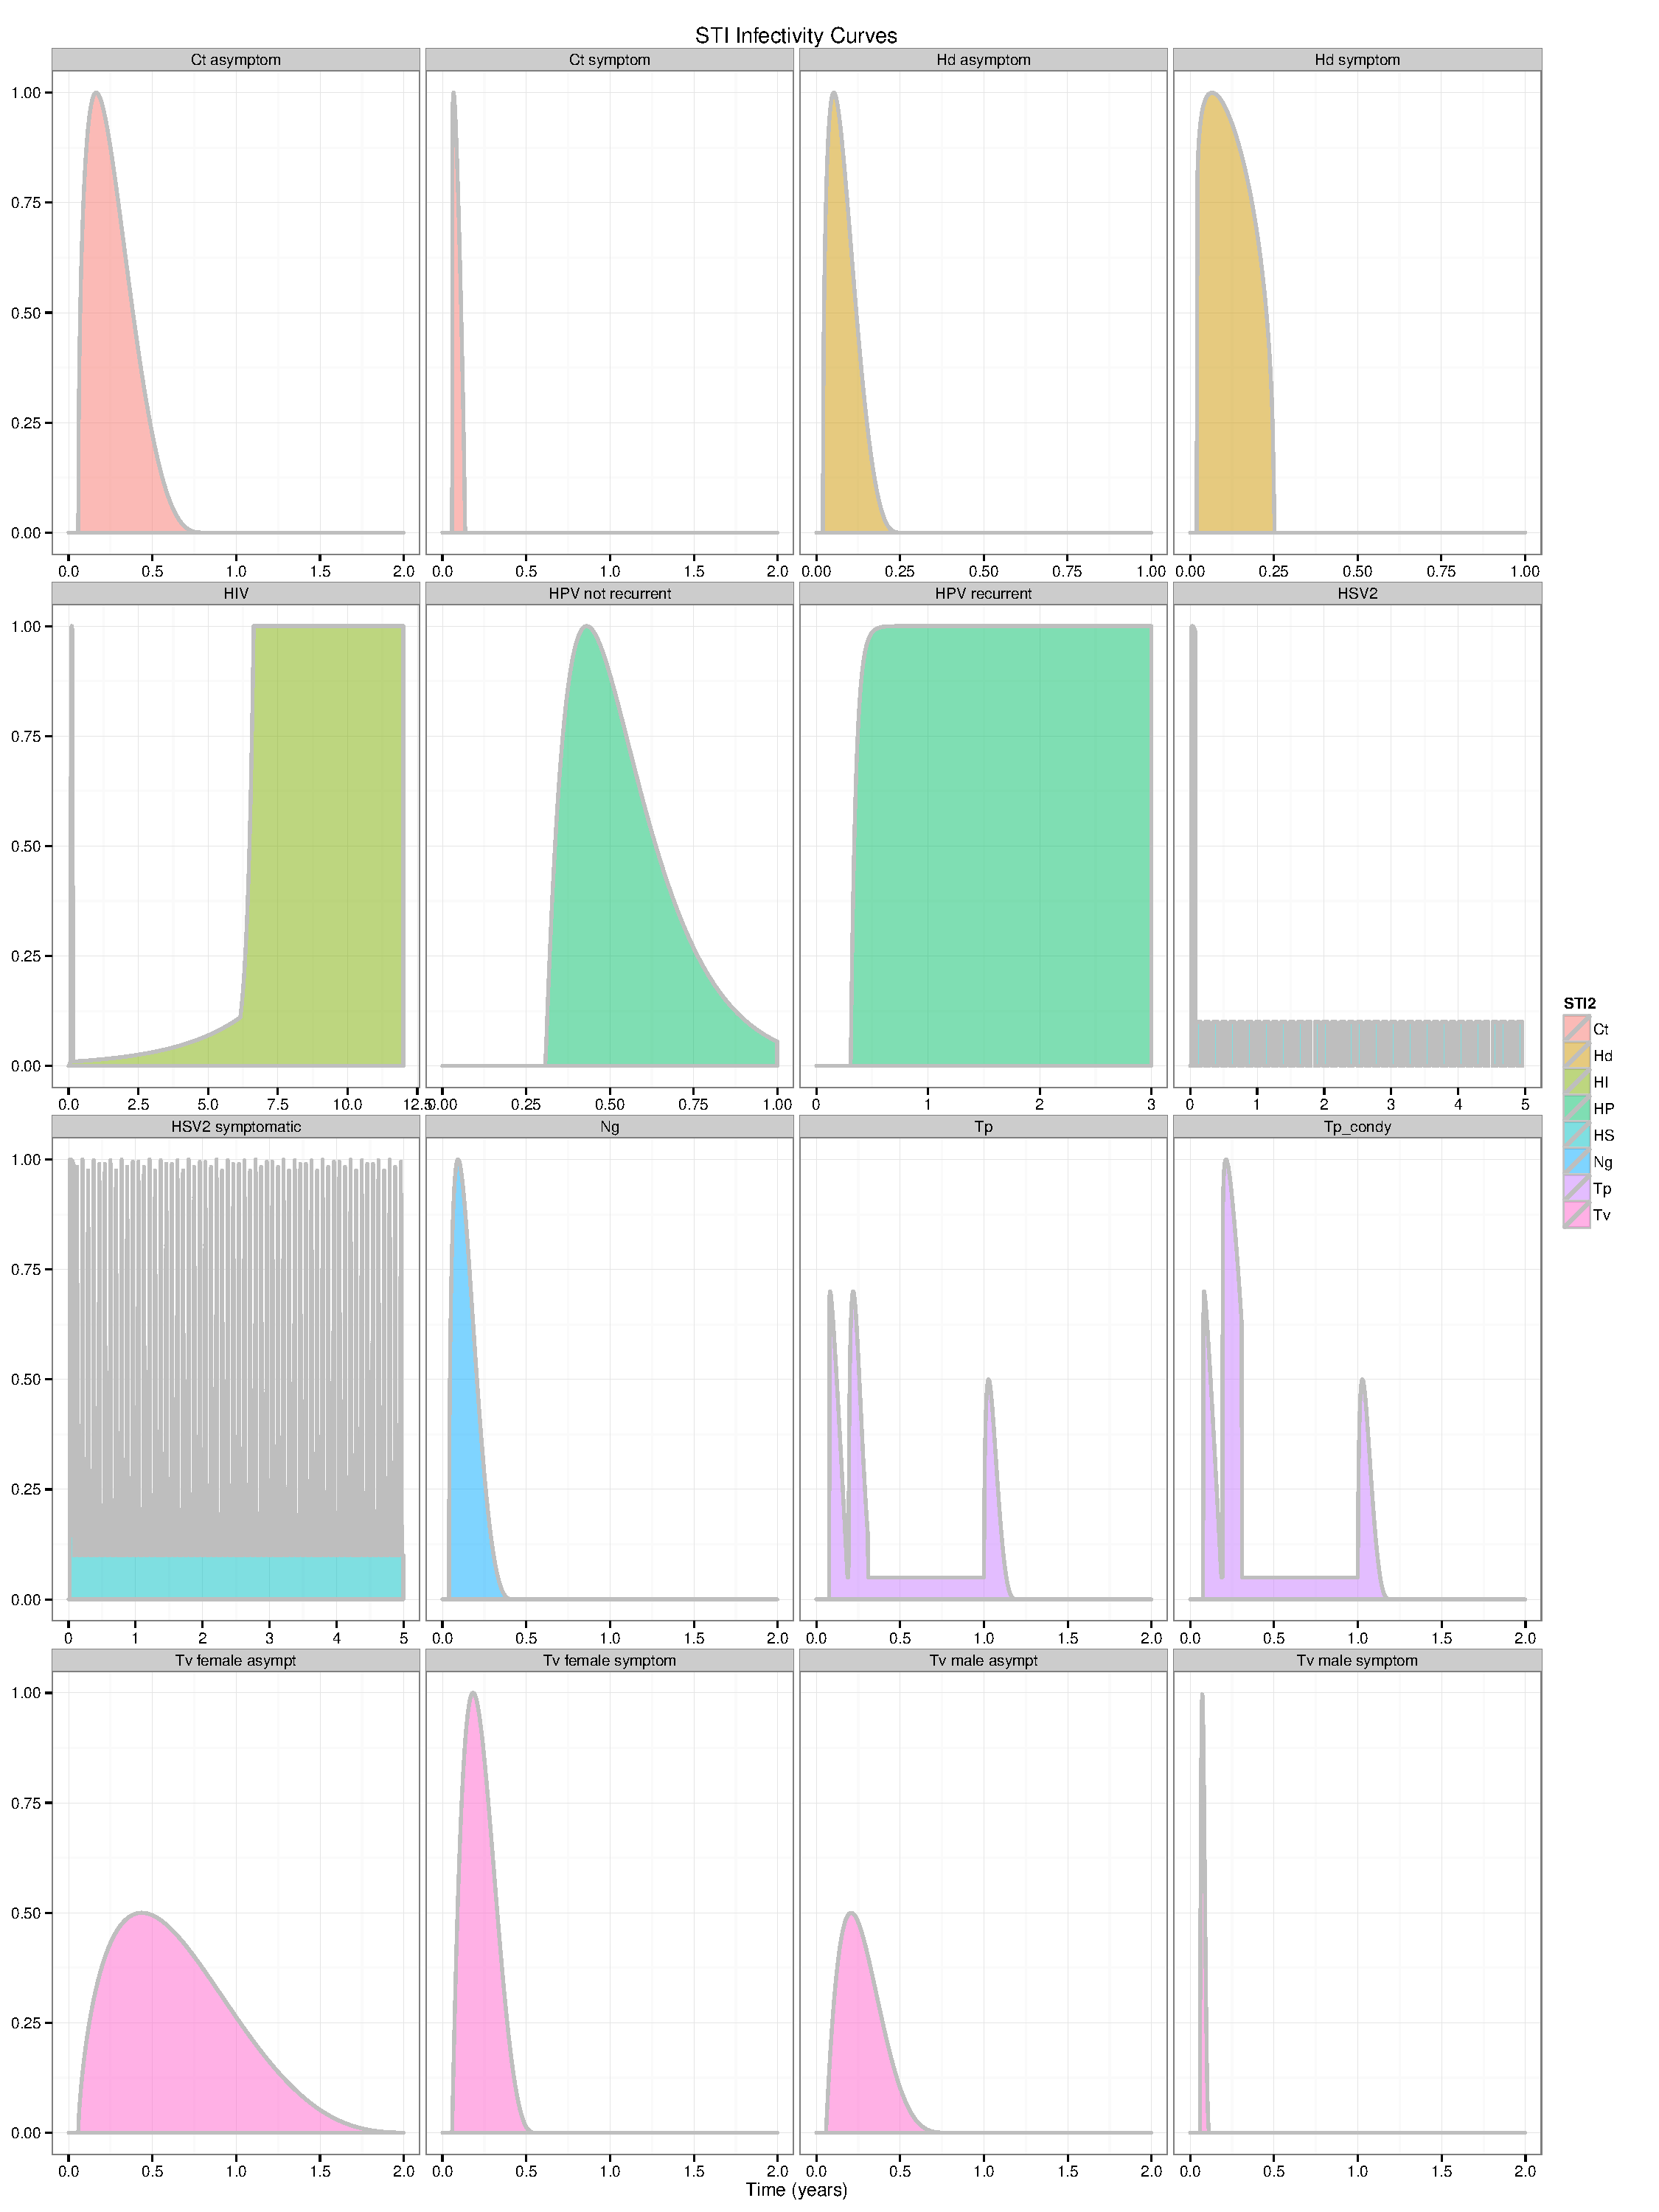
\includegraphics[angle=0,width=0.9\textwidth]{../CODECHECK/codecheck_STI_IC.pdf}
%\caption{Infectivity curves for each STI modelled.}
%\label{fig:InfectivityCurves}
%\end{figure}


\subsubsection{HSV2}
(reference: Tronstein 2011 \cite{Tronstein:2011vs}, Schiffer 2014 \cite{xxx})

An important feature in the natural history of HSV2 is whether the infection will be symptomatic (visible and/or painful lesions) or not.
Most of HSV2 infections are asymptomatic. This is set in the model at the time when the individual acquires the disease, by drawing a uniform random variable. Viral shedding is recurrent whether the infection is symptomatic or not, but the frequency and duration of viral shedding is longer when symptomatic \cite{Tronstein:2011vs}. 

It is assumed there is a small background viral shedding between recurrent lesions. Hence, the infectivity curve has a minimum value set at $vs_{min}v_{min}^{HSV2}$ to represent this minimum amount of viral shedding. 

The infectivity curve is defined in two pieces: a first representing the first ulcerative episode, the second representing the (potential) recurrence of lesions.
$$IC_{HSV2,first}(t) = (1-v_{min}^{HSV2})e^{-(t-L_{HSV2}-\frac{1}{2}D_{ulcer}^{HSV2})^2 / \sigma^{HSV2}_1}+v_{min}^{HSV2}$$

with $t$ the time since infection, $L_{HSV2}$ the latent period, $D_{ulcer}^{HSV2}$ the duration of the ulcerative episode and $\sigma^{HSV2}_1$ representing the dispersion of the infectiousness around the peak infectivity.
For the recurrent events, for $t \geq 2(L_{HSV2}+D_{ulcer}^{HSV2})$:

$$ IC_{HSV2,rec}(t) =  \frac{e^{\sin^2(\pi\omega t)/\sigma^{HSV2}_2}-1}{e^{1/\sigma^{HSV2}_2}-1}  (1-v_{min}^{HSV2})+ v_{min}^{HSV2}$$

with $\omega = \mathrm{sympt}\,\omega_s^{HSV2} + (1- \mathrm{sympt})\omega_a^{HSV2}$, $\sigma^{HSV2}_2 = \mathrm{sympt}\,\sigma_s + (1- \mathrm{sympt})\sigma_a$ and  $ \mathrm{sympt}$ a binary variable equal to 1 if the infection is symptomatic, 0 else; $\omega$ is the frequency of recurrence (expressed in events per year) and $\sigma^{HSV2}_2$ the dispersion of the duration of the recurrent lesion.

(suggested: $\omega_a^{HSV2}=12, \sigma_a=0.1, \omega_s^{HSV2}=1.5\omega_a^{HSV2}, \sigma_s=100\sigma_a, v_{min}^{HSV2}=0.1$) 

The final infectivity curve for HSV2 is given by
$$IC_{HSV2}(t) = IC_{HSV2,first}(t) + IC_{HSV2,rec}(t)   $$


Circumcision reduces HPV acquisition risk by about 30\% \cite{Tobian:2009kp}


\subsubsection{HPV}

Sources: \cite{Stanley:2011dd} \cite{Baussano:2013dh}


Incubation period ranges from 3 weeks to 8 months. Most (80-90\%) of HPV infections are cleared by the immune system after 4/8 months for low risk types or 8/16 months for high-risk types. If the immune response does not clear HPV infection, then a persistent infection is established.

Circumcision reduces HPV acquisition risk by about 35\% \cite{Tobian:2009kp}

Hence, the infectivity curve for HPV is implemented as follows. 

There is a stochastic latent period $L_{HPV}$ before which the individual is not infectious. It is assumed that there is a maximum latent period $L_{HPV}^*$ (deterministic constant - suggestion: 8 months) and the distribution:
$$L_{HPV} \sim L_{HPV}^* \times \mathrm{Beta}(3,3) $$

So, the infectivity curve during the latent period is obviously
$$IC_{HPV}(t< L_{HPV}) = 0$$

A random variable, distributed as $Bern(p_{HPV})$, determines if the HPV infection will be persistent or not (suggestion: proba persistence $p_{HPV}$ = 10\%)

The infectivity curve is then defined as
$$IC_{HPV}(t) = t' e^{-k_{hpv}\, t' }/ \eta_0$$

with $t' = (t-L_{HPV})/D_{HPV} $, $D_{HPV}$ the duration of infectiousness, $k_{hpv}$  a shape parameter (suggestion: $k_{hpv}=5$) and $\eta_0=e^{-1}/k_{hpv}$ the normalizing constant.

If HPV will be persistent, then 
$$IC_{HPV}(t) = 1- e^{-t'/\eta_0 }$$
(shape was chosen such that it has the same initial slope as the non-persistent case)

The resulting infectivity curve for HPV are represented in Figure \ref{fig:ICHPV}.
\begin{figure}[!ht]
\centering
    \includegraphics[angle=0,width=0.8\textwidth]{./infectivity_curves/IC_HPV.pdf}
\caption{Infectivity curve for HPV. Dash line represent persistent infection.}
\label{fig:ICHPV}
\end{figure}



\subsubsection{Chlamydia (Ct)}

Sources: \cite{Geisler:2010bc, Althaus:2011dc}. \warning{also compare with \cite{Hontelez:2013bc} \cite{Althaus:2012gg}}

Chlamydia clearance rate after 1 year of infection is about 50\%, 80\% after 2 years and 90\% after 3 years \cite{Geisler:2010bc}.

Average incubation period is about 2 weeks and about 25\% of cases will be symptomatic \cite{Althaus:2011dc}. There are lower estimates for the proportion of symptomatic cases at 10\% for men, 6\% for women \cite{Korenromp:2002gt}; and higher estimates with 75\% symptomatic for men and 30\% for women \cite{Kretzschmar:1996ur}.

\warning{Implement?: Korenromp\cite{Korenromp:2002gt} finds a much larger duration of infection for women than men... INVESTIGATE!}

Infectious period seems to depend on symptomatic status: 6-12 months when asymptomatic, but about 1 month when symptomatic\cite{Kretzschmar:2009cd}.

Symptomatic status is determined by a (stochastic) bernoulli variable $sympt\sim Bern(p_{Ct})$, with $p_{Ct}$ being the probability that a chlamydia infection will be symptomatic for a given individual (suggestion: $p_{Ct}=0.2$).

If $L_{Ct}$ is the duration of the latent period, $a_{Ct}$ and $b_{Ct}$ shape parameters and $D_{Ct}$ the infectious period, the infectivity curve for chlamydia is
$$IC_{Ct}(t) = \mathcal{B}\left(\frac{(t-L_{Ct})^+}{D_{Ct}},a_{Ct},b_{Ct}\right)$$

If the infection is symptomatic, the shape parameters are changed and the duration of infection is shorten
$$IC_{Ct,sympt}(t) = \mathcal{B}\left(\frac{(t-L_{Ct})^+}{D_{Ct.s}},a_{Ct.s},b_{Ct.s}\right)$$

\begin{figure}[!ht]
\centering
    \includegraphics[angle=0,width=0.8\textwidth]{./infectivity_curves/IC_Ct.pdf}
\caption{Infectivity curve for Chlamydia. Dash line represents asymptomatic infection.}
\label{fig:ICCt}
\end{figure}



\subsubsection{Neisseria Gonorrhoeae (Ng)}

 Symptomatic in most of men ($> 90\%$\cite{Ison:2011eg,Kretzschmar:1996ur}, 50\%\cite{Korenromp:2002gt} ), but not in women ($< 50\%$\cite{Ison:2011eg,Kretzschmar:1996ur}, 15\%\cite{Korenromp:2002gt}) 
 
 Incubation time: 1-2 weeks\cite{Kretzschmar:1996ur}
 
 Duration of infection: 4-6 months \cite{Chen:2010hx,Korenromp:2002gt}
 
 The infectivity curve is similar to Chlamydia's one:
$$IC_{Ng}(t) = \mathcal{B}\left(\frac{(t-L_{Ng})^+}{D_{Ng}},a_{Ng},b_{Ng}\right)$$
with $L_{Ng}$ the latent period (suggested: 1 week), $D_{Ng}$ duration of infection (suggested 5 months) and $a$ and $b$ shape parameters.
\begin{figure}[!ht]
\centering
    \includegraphics[angle=0,width=0.8\textwidth]{./infectivity_curves/IC_Ng.pdf}
\caption{Infectivity curve for Gonorrohea.}
\label{fig:ICNg}
\end{figure} 
 
 
 \subsubsection{Syphilis (Treponema pallidum, Tp)}

Primary syphilis: After initial exposure, a primary chancre develops at the site of entry (usually genital) after 3-90 days (average 3 weeks) \cite{Kent:2008ch,Horvath:2011fw}. It takes about 4-6 weeks for spontaneous resolution (without treatment) of the primary chancre.

Secondary syphilis: Up to 85\% of cases will progress to generalized lesions\cite{Horvath:2011fw}, within 4-10 weeks after the appearance of the initial chancre\cite{Kent:2008ch,Horvath:2011fw}. A small proportion of cases, 10\%\cite{Horvath:2011fw} 5-22\%\cite{Kent:2008ch}, will develop highly infectious chancres (condylomata lata). Spontaneaous resolution occurs within less than 3 months\cite{Horvath:2011fw} or several weeks\cite{Kent:2008ch}.

Early latent syphilis: About 25\% of cases experiences a recurrence of secondary syphilis symptoms during a window period of about 6 months

Syphilis (untreated) is expected to be sexually transmissible during 2 years after initial infection\cite{Horvath:2011fw}. Late latent and tertiary phases are not infectious. Tertiary phase occurs 15-30 years later and is associated with increased mortality in some cases. 

Co-infection with HIV might be associated with a higher Tp virulence, but syphilis treatment is the same as HIV-uninfected patients\cite{Kent:2008ch}.\warning{not sure if Tp's IC should be significantly affected by HIV co-infection... probably yes}

The infectivity curve is defined with respect to the syphilitic stages.

Primary syphilis infectivity curve is represented with the pseudo-beta function defined in section \ref{sec:pseudo beta}:
$$IC_{Tp.1}(t) = v_{Tp.1}\times\mathcal{B} \left(\frac{(t-L_{Tp.1})^
+}{D_{Tp.1}}, a_{Tp.1},b_{Tp.1} \right) $$
with $a_{Tp.1}$ and $b_{Tp.1}$ shape parameters (suggested $a_{Tp.1}=1.5$, $b_{Tp.1} = 4$), $L_{Tp.1}$ the latent period before being infectious (suggested 30 days), $D_{Tp.1}$ the infectiousness duration of primary syphilis (suggested 5 weeks) and $v_{Tp.1}$ the relative virulence of this primary stage (suggested 0.7) compared to peak infectivity (when the value of the infectivity curve is 1).

Secondary syphilis is defined similarly, but with two possibilities for the infectivity curve reflecting the fact that some cases will develop highly infectious condylomata lata.

In the absence of condylomata:
$$IC_{Tp.2}^{no\,condy}(t) = v_{Tp.2}\times\mathcal{B} \left(\frac{(t-L_{Tp.2})^
+}{D_{Tp.2}}, a_2,b_2 \right) $$
when condylomata develop:
$$IC_{Tp.2}^{condy}(t) = v_{Tp.2}^{condy}\times\mathcal{B} \left(\frac{(t-L_{Tp.2})^
+}{D_{Tp.2}^{condy}}, a_2^{condy},b_2^{condy} \right) $$

with $a_2$ and $b_2$ shape parameters (suggested $a_2=a_1$, $b_2 = b_1$ \warning{double check}), $L_{Tp.2}$ the latent period from infection before secondary syphilis is triggered(suggested $L_{Tp}$ plus 7 weeks), $D_{Tp.2}$ the infectiousness duration of secondary syphilis (suggested 8 weeks) and $v_{Tp.2}$ the relative virulence of this secondary stage (suggested 0.7) compared to peak infectivity. 

The parameters with the superscript $condy$ apply to the case when condylomata develop. In this case, the parameters are assumed to be different:  $a_2^{condy}=1.1$, $b_2^{condy}=1.8$,$ v_{Tp.2}^{condy}=1$

The probability that condolymata develop is represented by the binary random variable $\kappa_{condy}$ that takes value 1 with probability $p_{condy}$ (suggested 0.15), else is 0.

Hence, for secondary syphilis we have:
$$IC_{Tp.2}(t)  = \kappa_{condy}IC_{Tp.2}^{condy}(t) +(1-\kappa_{condy})IC_{Tp.2}^{no\,condy}(t) $$

Early latent syphilis is considered as a repeat of symptoms that occurred during secondary syphilis, hence it is defined similarly:

$$IC_{Tp.el}(t) = v_{Tp.el}\times\mathcal{B} \left(\frac{(t-L_{Tp.el})^
+}{D_{Tp.el}}, a_{el},b_1{el} \right) $$
with $a_{el}$ and $b_{el}$ shape parameters (suggested $a_{el}=a_2$, $b_{el} = b_2$), $L_{Tp.el}$ the latent period before earl latent stage is triggered (suggested $L_{Tp}$ plus 12 months), $D_{Tp.1}$ the infectiousness duration of primary syphilis (suggested 5 weeks) and $v_{Tp.el}$ the relative virulence of this primary stage (suggested 0.5 \warning{double check}) compared to peak infectivity.

Finally, the total infectivity curve for syphilis is:
$$IC_{Tp.el}(t) = IC_{Tp.1}(t) +\kappa_{Tp.2}IC_{Tp.2}(t) +\kappa_{Tp.el}IC_{Tp.el}(t) $$
with $\kappa_{Tp.2}$ (resp. $\kappa_{Tp.el}$ ) the binary random variable taking value 1 with probability $p_{Tp.2}$ (resp. $\kappa_{Tp.el)}$ representing the probability to develop secondary (resp. early latent) syphilis. (suggested: $p_{Tp.2}=0.85$ and $\kappa_{Tp.el}=0.20$)

A graphical representation is given in Figure \ref{fig:ICTp}

\begin{figure}[!ht]
\centering
    \includegraphics[angle=0,width=0.8\textwidth]{./infectivity_curves/IC_Tp.pdf}
\caption{Infectivity curve for Syphilis. The thin curve in the secondary syphilis stage represents the case when highly infectious condolymata develop.}
\label{fig:ICTp}
\end{figure} 

\subsubsection{Chancroids (Hd)}

 Incubation period is 4-7 days, rarely less than 3 days or more than 10 days \cite{Sakuma:2011gx,Morse:1989io}. The first symptoms are pustules (which are often not noticed by patients), then painful ulcers develop within a few days to 2 weeks \cite{Sakuma:2011gx} after the pustules. Pustules may resolve spontaneously or last several weeks\cite{Spinola:2002kn}. Chancroid symptomatic mostly in men (ratio men to women is from 3:1 to 25:1) \cite{Sakuma:2011gx} and pustules formation is more likely in men than in women (OR=2 \cite{Spinola:2002kn}).
Circumcision seems protective \cite{Hammond:1980uz}. Transmission rate is unknown but is believed to be high \cite{Spinola:2002kn}. 

Treatment takes between 1 and 2 weeks to completely clear the infection. Some strains may be antibiotics resistant.


The shape of the infectivity curve is supposed to be similar to the Chlamydia's, that is
$$IC_{Hd}(t) = \mathcal{B}\left(\frac{(t-L_{Hd})^+}{D_{Hd}},a_{Hd},b_{Hd}\right)$$

$$IC_{Hd,sympt}(t) = \mathcal{B}\left(\frac{(t-L_{Hd})^+}{D_{Hd.s}},a_{Hd.s},b_{Hd.s}\right)$$

\begin{figure}[!ht]
\centering
   \includegraphics[angle=0,width=0.8\textwidth]{./infectivity_curves/IC_Hd.pdf}
\caption{Infectivity curve for Chancroid (Hd). Dash line represents asymptomatic infection.}
\label{fig:ICHd}
\end{figure}


The latent period $L_{Hd}$ is assumed to be 1 week (same for both symptomatic or not), and the duration of infectiousness $D_{Hd}$ and $D_{Hd.s}$ (when symptomatic) are both equal to 3 months


\subsubsection{Trichomoniasis (Tv)}

(extensive but old review by Jirovec \cite{Jirovec:1968vi})

It is believed most men infected with Tv are asymptomatic, whereas a majority of women are symptomatic \cite{Pellicane:2011dk,Schwebke:2004bq}. However, there seems to be a large variability and studies' findings are controversial, especially regarding men \cite{Krieger:1995ur}. There are also reports of asymptomatic cases becoming symptomatic after 6 months \cite{Petrin:1998te}.

Incubation is often reported to be between 3 to 28 days, at least for 50\% of cases \cite{Petrin:1998te}. However, there seems to be some variability: while most of cases (60\% or more) have an incubation period less than 10 days for men, it could go as far as 3 months \cite{Krieger:1995ur}. There is no data on the latent period, so it is assumed to be at least 10 days.

Duration of infection is believed to be less than 10 days \cite{Petrin:1998te}, but here again seems highly variable and some reports to be as long as 3 months \cite{Krieger:1995ur}. Among men, infection seems to be cleared after 2 weeks in most cases (70\%) \cite{Krieger:1995ur}. Among women, untreated Tv infection is believed to last 3 months on average \cite{Pellicane:2011dk}.
There is no data on the duration of infectiousness so it is assumed to be the same as the duration of infection.


There is no immunity protection provided by previous Tv infections.

The probability to be symptomatic is set at 40\% for males and 80\% for females.

There are controversial report on the protective effect of male circumcision regarding Tv infection: one study \cite{Mehta:2009bh} did not find any association, whereas another \cite{SobngwiTambekou:2008fs} found one (OR=0.5). We assume a protective effect of 0.75. 

The infectivity curve for Tv is segregated by gender and symptomatic status. For symptomatic individuals we have:
$$IC_{Tv}^{\,g,a}(t) =  \rho_{\,Tv}^g \times\mathcal{B}\left(\frac{(t-L_{Tv})^+}{D_{Tv.g.a}},a_{Tv.g.a},b_{Tv.g.a}\right)  $$
with $g=\{m,f\}$ the gender of the individual considered, $\rho_{\,Tv}^g$ the infectiousness reduction factor ($<1$) for asymptomatic cases, the latent period $L_{Tv}$ assumed to be the same value of 1 week for any case, $D_{Tv.g.a}$ duration of infection, $a_{Tv.g.a}$ and $b_{Tv.g.a}$ shape parameters. 

Similarly, for symptomatic cases:
$$IC_{Tv}^{\,g,s}(t) = \mathcal{B}\left(\frac{(t-L_{Tv})^+}{D_{Tv.g.s}},a_{Tv.g.s},b_{Tv.g.s}\right)  $$

Values for different cases (male/female and symptomatic or not) are given in Table \ref{tab:STIAllParamProtozoa} and illustrated in Figure \ref{fig:ICTv}.

\begin{figure}[!ht]
\centering
   \includegraphics[angle=0,width=0.8\textwidth]{./infectivity_curves/IC_Tv.pdf}
\caption{Infectivity curve for Trichomanas vagionisis (Tv). Dash line represents asymptomatic infection.}
\label{fig:ICTv}
\end{figure}


\subsubsection{Bacterial vag (Bv)}
\warning{not implemented (not considered as STI)}

\subsection{Mother to child transmission (MTCT)}

Every time a pregnancy is initiated, the probability of vertical transmission of all STIs the mother has is evaluated. This probability depends on the STI and the duration since infection. If vertical transmission occurs, it is recorded in the `nursery'.

The MTCT probabilities are defined here:

\begin{table}[htdp]
\caption{MTCT probabilities ($d$: duration of infection)}
\begin{center}
\begin{tabular}{|c|c|}
\hline
STI & Probability \\
\hline
HIV & 0.95 \\
Tp & $0.9/\left(1+e^{3(d-2)}\right)$  \\
\hline
\end{tabular}
\end{center}
\label{default}
\end{table}%



%%%%%%%%%%%%%%%%%%%%%%%%%%%%%%%%%%%%%%%%%%%%%
%%%%%%%%%%%%%%%%%%%%%%%%%%%%%%%%%%%%%%%%%%%%%

\section{Treatment}


\subsection{Generic implementation}

When an individual is infected with an STI, receiving a treatment will most likely reduce her/his infectiousness, symptomatic status and increase the chances of being cleared from the pathogen, if the STI is curable.

An individual starting a treatment will go through several steps before potentially having a positive outcome. 

\subsubsection{Treatment microbiological failure}

There is a risk of failure with any treatment. An individual may poorly respond to prescribed drugs, or be infected with a drug-resistant strain of the pathogen (adherence is treated separately hereafter).

For a given STI, let $TMS$ be the random variable representing microbiological treatment success (conditional on full adherence) and $p_{fail}$ the probability of treatment failure. It is assumed that $TMS$ has a Bernoulli distribution (1 is successful treatment):
$$TMS \sim \mathrm{Bern}(1- p_{fail})$$

\warning{insert a table with the $p_{fail}$ for each STI}

\subsubsection{Adherence}
\warning{NOT PROPERLY IMPLEMENTED YET!}\\
Right from treatment inception, adherence is determined based on the individual's risk group and symptomatic status and the optimal treatment duration noted $TD^*$ \warning{OTHERS???}. A non-adherent behaviour will reduce the amount of drug intake. If adherence $A$ is measured as the fraction of the optimal drug intake ($0 \leq A\leq 1$, with $A=1$ being full adherence), then it is assumed
$$ A \sim \mathrm{Beta}(a_1; a_2)$$
with $a_1$ and $a_2$ being parameters function of the STI considered, $TD^*$ and the risk group and symptomatic status \warning{(others?)} of the infected individual.


\subsubsection{Treatment reduction effect}

Treatment is affecting the infectivity curve, with the aim of reducing it to either 0 for curable STI or a very small value for non-curable STIs. 

We assume there is an hypothetical treatment reduction effect ($TRE^*$) conditional on microbiological success and full adherence. It is a function of treatment duration $\tau$ and we have $TRE^*(0)=1$ (no reduction of infectiousness at the very start of treatment) and $TRE^*(TD^*)=0$ or $\epsilon$ (treatment has cured [when STI is curable] or heavily suppressed [when non-curable] the pathogen). The actual treatment reduction effect $TRE$ is given by
$$TRE(A, TMS,\tau) = \left[A\times TRE^*(\tau) + (1-A) \right] TMS + (1-TMS) $$

Function $TRE^*$ will be defined specifically for each STI.

\begin{figure}[!ht]
\centering
    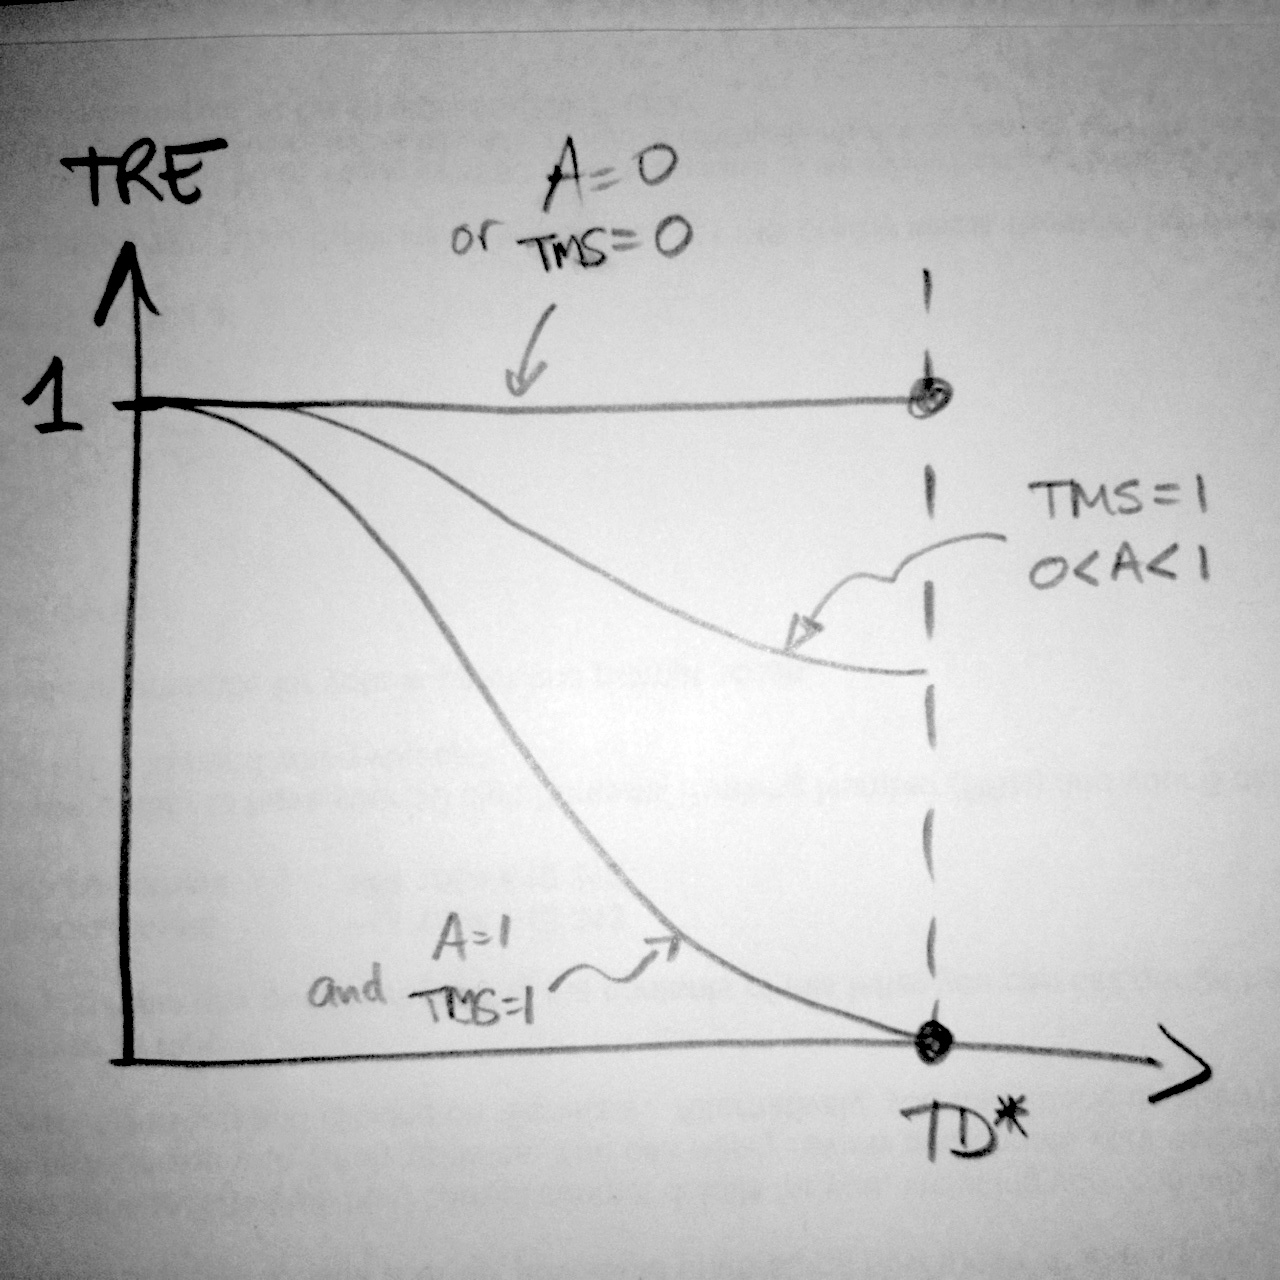
\includegraphics[angle=0,width=0.5\textwidth]{TRE.JPG}
\caption{Treatment reduction effect.}
\label{fig:TRE}
\end{figure}

The infectivity curve before treatment ($IC$) is thus modified into an infectivity curve during treatment ($IC^{treat}$):
$$IC^{treat}(t,\tau)= IC(t)\times TRE(A,TMS,\tau)  $$

For curable STIs, cure is achieved if all of the conditions below are met
\begin{itemize}
\item There is a microbiological success ($TMS=1$, that is no resistance etc)
\item treatment duration is greater than optimal treatment duration ($\tau>TD^*$)
\item adherence is larger than 50\% ($A>0.5$) 
\end{itemize}


\subsection{Treatment each STI}

\subsubsection{Bacterial STIs}
\subsubsection{Viral STIs}



%%%%%%%%%%%%%%%%%%%%%%%%%%%%%%%%%%%%%%%%%%%%%
%%%%%%%%%%%%%%%%%%%%%%%%%%%%%%%%%%%%%%%%%%%%%

\section{Vaccination}



%%%%%%%%%%%%%%%%%%%%%%%%%%%%%%%%%%%%%%%%%%%%%
%%%%%%%%%%%%%%%%%%%%%%%%%%%%%%%%%%%%%%%%%%%%%



%%%%%%%%%%%%%%%%%%%%%%%%%%%%%%%%%%%%%%%%%%%%%
%%%%%%%%%%%%%%%%%%%%%%%%%%%%%%%%%%%%%%%%%%%%%

\section{Migrations between populations}
[[ Not implemented yet ]]


%%%%%%%%%%%%%%%%%%%%%%%%%%%%%%%%%%%%%%%%%%%%%
%%%%%%%%%%%%%%%%%%%%%%%%%%%%%%%%%%%%%%%%%%%%%

\section{Simulation}

\warning{THIS SECTION IS NOT CLEANED}

\subsection{Calibration}

\subsubsection{Newest stuff (feb-2015)}

There is a concept of calibration schedule: various response variables are targeted at various points of time during the simulation.


\begin{figure}[!ht]
\centering
    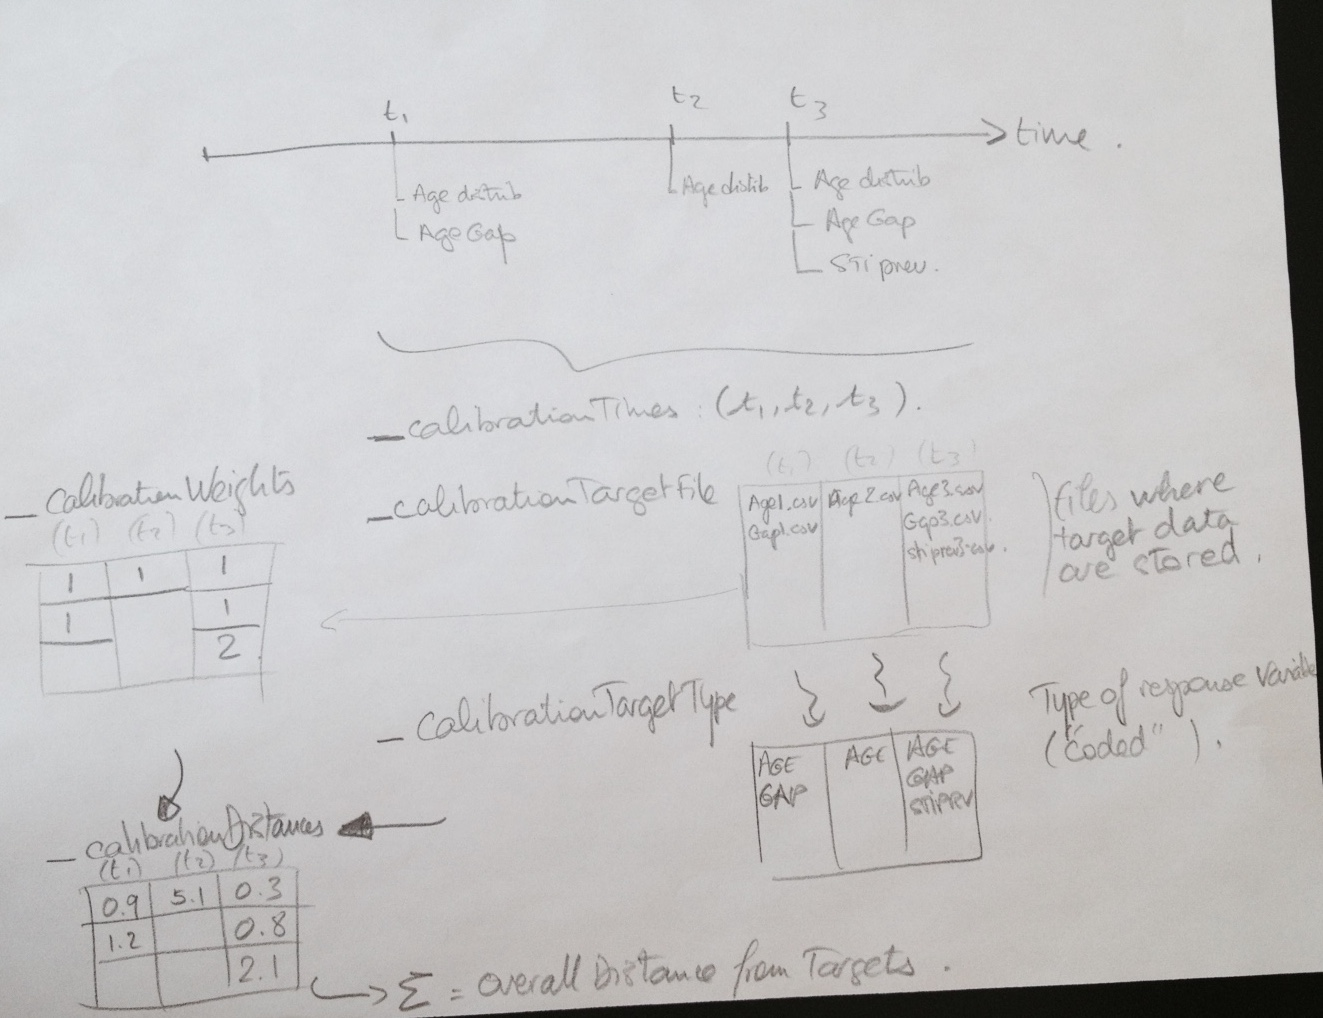
\includegraphics[angle=0,width=0.9\textwidth]{calibration_schedule.jpg}
\end{figure}


\subsubsection{Response variable of the Model to be calibrated}

\warning{look at SPSA algorithm for stochastic optimization}

Several key quantities are observable or have been estimated, and relevant parameters of the model are calibrated to these ``target quantities''.
\begin{table}[htdp]
\caption{Response variables to be calibrated}
\begin{center}
\begin{tabular}{lll}

\hline
\textbf{Category} & \textbf{Target Quantity} & \textbf{Parameters} \\

\hline
Demographic  &  Age structure & Birth rates, death rates (Weibull parameters)\\
 & & (STI prevalence when HIV modelled)\\
\hline
Partnerships  &  Ratio \#singles/total population  &  Formation/dissolution rates and preferences \\
  &  Age gaps &   Formation/dissolution rates and preferences  \\
  &  Spousal ratio & Spousal preferences \\
 & & (STI prevalence when HIV modelled)\\
\hline
STIs	& Global prevalence & Demographics, partnerships,\\
	& Prevalence by risk group & STI infectivity/susceptibility,\\
	& Prevalence by age & CSW and sex behaviour\\
\hline
\end{tabular}
\end{center}
\label{default}
\end{table}


Source for the target level of the response variable varies between countries. Agencies (e.g. UN, WHO, DHS) is a good source of data at the  country level, and peer-reviewed publications have data at a finer level.

Not all parameters of this model need to be calibrated. Fairly good historical estimations are available for some of them (UN, DHS, etc), hence they will be used. 

The objective function to minimize can be expressed as $F(X)$, with $X$ is the vector of all parameters to be calibrated such that the response variables are the closest to their respective target.
\begin{eqnarray*}
F(X) & =&\,\omega_{AD}(AgeDist - target_{AD})^2 \\
& & + \omega_{PR}(PartnerRatio - target_{PR})^2 \\
& & + \omega_{AG}(AgeGap - target_{AG})^2 \\
& & +\sum_s \omega_{TP}(STItotPrev_s-target_{TP,s})^2 \\
& & +\sum_s \omega_{RGP}(STIRiskGrpPrev_s-target_{RGP,s})^2\\
& & +\sum_s \omega_{AP}(STIAgePrev_s-target_{AP,s})^2
\end{eqnarray*}
with $\omega$ calibration weights \warning{((ARBITRARY VALUE??))}. 

We search $X^*$ such that $F(X^*)=\min_{X\in \mathcal{A}} F(X)$, where $\mathcal{A}$ is the parameter space delimited by predfined lower and upper bounds.

\subsubsection{Algorithm (high-level)}
The calibration to current data is actually made in 3 high level steps

\textbf{Step 1: Fitting to pre-HIV era}

Population initialized with data ``well before'' the HIV epidemic starts:
\begin{itemize}
\item Rough age distribution
\item No partnerships
\item Rough STIs prevalence (no HIV)
\end{itemize}

Simulation is run for as long as necessary to reach the time $T_{HIV}$ just before the HIV epidemic starts. The dynamics of the population is supposed to reach an equilibrium regime where age distribution, partnerships distributions (age gaps, proportion of spousal partnerships, etc) and STIs prevalences must be calibrated to data prevalent at time  $T_{HIV}$.

\textbf{Step 2: HIV is introduced in the population}

A small proportion of HIV infections is introduced in the population [DECIDE HOW MORE PRECISELY].

\textbf{Step 3: Fitting to today's data}

The simulation is run for a duration that equals the length of the HIV epidemic in the location considered. Then, at the time horizon (:today) of the simulation, partnerships distributions and STIs and HIV prevalences must be calibrated to the latest data.

Then, the model is assumed to be fitted and simulation in the future can be run.








\section{Miscellaneous Notes}

\subsection{Pseudo-beta shape function} \label{sec:pseudobeta}

For infectivity curves associated with STIs of limited duration, the shape function was inspired from the beta distribution density (because it has a bounded support).
$$\mathcal{B}(x,a,b) = x^{a-1}(1-x)^{b-1}/C$$
where $C$ is the normalizing constant such that the maximum value of $\mathcal{B}$ is 1 on the interval [0;1]:
$$C=\left(\frac{a-1}{a+b-2}\right)^{a-1}\left(\frac{b-1}{a+b-2}\right)^{b-1}$$
It is assumed that for any $a,b>1$ and  $x<0$ and $x>1$ we have $\mathcal{B}(x,a,b)=0$.
The maximum of $\mathcal{B}$ is reached at $x_{max}=(a-1)/(a+b-2)$.


\newpage



\section{Model Parameters Summary}

%\begin{landscape}

%%%%% DEMOGRAPHICS TABLE %%%%

\begin{table}[htdp]

\begin{footnotesize}
\begin{center}
\begin{tabular}{|clc|}
\hline
\textbf{Parameter}  & \textbf{Description} & \textbf{Baseline Value}\\
\hline

\textbf{Demographics} & & \\
 birthRate & Crude birth rate for the whole population & calibrated\\
$\alpha$  & blabla & 0.2 \\
$\beta$  & blabla & 0.23 \\
\hline
\end{tabular}
\caption{Exhaustive list of all model parameters related to demographics}
\label{tab:demogAllParam}
\end{center}
\end{footnotesize}
\end{table}


%%%%% PARTNERSHIP TABLE %%%%

\begin{table}[htdp]

\begin{footnotesize}
\begin{center}
\begin{tabular}{|clc|}
\hline
\textbf{Parameter}  & \textbf{Description} & \textbf{Baseline Value}\\
\hline

\textbf{Formation} & & \\
 $\varphi_f$ & Average formation rate (female dominance) & calibrated (1.5 year$^{-1}$)\\
$s_{f_\mathrm{age}}$  & Shape parameter for age gap of partnership formation & calibrated (0.015)\\
$\bar{a}_{f_\mathrm{age}}$  & Mean age of partnership formation for females & calibrated \\
$\sigma_{a_f}$  & Variance of age for partnership formation for females & calibrated \\
$\bar{g}_{f_\mathrm{age}}$  & Mean age gap of partnership formation & calibrated \\
$\sigma_{g_f}$  & Variance of age gap for partnership formation & calibrated  \\
$\rho_f$  & Correlation b/w female age and age gap for partnership formation & calibrated  \\
$s^{\mathrm{risk}}_0$ ; $s^{\mathrm{risk}}_1$  & Shape parameters for risk group assortativity & calibrated  \\
\textbf{Dissolution} & & \\
$d_{\mathrm{spouse}}$&Probability reduction to dissolve a spousal partnership & calibrated\\
$g_{deficit,min}$ & Maximum reduction of dissolution probability die to partnership deficit& calibrated\\
 $q_{deficit}$ & Shape parameter involved in the dissolution probability & calibrated \\


\hline
\end{tabular}
\caption{Exhaustive list of all model parameters related to parterships}
\label{tab:partnerAllParam}
\end{center}
\end{footnotesize}
\end{table}


%%%%% STI TABLE -- VIRUS %%%%

\renewcommand{\arraystretch}{1.25}
\begin{table}[htdp]

\begin{scriptsize} %tiny %scriptsize % \footnotesize

\begin{center}
\begin{tabular}{|clc|}
\hline
\textbf{Parameter}  & \textbf{Description} & \textbf{Baseline Value}\\
\hline
\hline
\textbf{HIV} & & \\
\hline
$Tvl^*_{HIV}$ & Time after initial infection when viral load peaks & 6 weeks\\
$q_{HIV}$ & Shape parameter of acute infection & 2 \\
$\sigma_{HIV}$ & Dispersion of the duration of acute phase & 2 weeks \\
$VL_{chronic}$ & Fraction of peak viral load when chronic stage starts  & $10^{-2}$ \warning{Saturation? see Williams 2011}\\
$D_{chronic}$ & Duration (in years) of the chronic infectious stage & 7 years \\
$r_{chronic}$ & Rate of viral load progression during the chronic stage & 0.4 \warning{[[AGE DEPENDENT?]]}\\
$D_{AIDS}$ & Duration (in years) of AIDS (death as end-point) & 1.5 years \\
\hline
\textbf{HSV2} & & \\
\hline
$v_{min}^{HSV2}$ & Minimum value of HSV2 infectivity curve & 0.1\\
$L_{HSV2}$ & Latent period for HSV2 & 1 week\\
$D_{ulcer}^{HSV2}$ & duration of the ulcerative episode & 1 week\\
$\sigma^{HSV2}_1$ & dispersion of HSV2 infectiousness around peak infectivity & ??\\ 
$\sigma^{HSV2}_{2,a}$ & dispersion of the duration of the recurrent lesion, asymptomatic& ??\\ 
$\sigma^{HSV2}_{2,s}$ & dispersion of the duration of the recurrent lesion, symptomatic& ??\\ 
$\omega_a^{HSV2}$ & frequency of recurrence for asymptomatic HSV2 & 12 events/year\\
$\omega_s^{HSV2}$ & frequency of recurrence for symptomatic HSV2 & 18 events/year\\
\hline
\textbf{HPV} & & \\
\hline
$L_{HPV}$ & Latent period for HPV & 6 months\\
$p_{HPV}$ & Probability of HPV persistence & 0.1\\
$D_{HPV}$ & Duration of HPV infectiousness (per episode) & 1 week\\
$k_{hpv}$  & Shape parameter for HPV infectivity curve & 5.0 \\
\hline

\end{tabular}
\caption{Exhaustive list of all model parameters related to viral STIs}
\label{tab:STIAllParamVirus}
\end{center}
\end{scriptsize}
\end{table}



%%%%% STI TABLE -- Bacteria %%%%

\renewcommand{\arraystretch}{1.25}
\begin{table}[htdp]

\begin{scriptsize} %tiny %scriptsize % \footnotesize

\begin{center}
\begin{tabular}{|clc|}
\hline
\textbf{Parameter}  & \textbf{Description} & \textbf{Baseline Value}\\
\hline
\hline
\textbf{Syphilis} & & \\
\hline
$v_{Tp.1}$ & primary syphilis virulence (relative to peak) & 0.7\\
$a_{Tp.1}$ &  shape parameter primary syphilis & 1.5\\
$b_{Tp.1}$ &  shape parameter primary syphilis & 4\\ 
$L_{Tp.1}$ &  latent period primary syphilis & 4 weeks\\
$D_{Tp.1}$ &  infectiousness duration primary syphilis & 5 weeks\\
$v_{Tp.2}$ & secondary syphilis virulence (relative to peak) & 0.7\\
$a_{Tp.2}$ &  shape parameter secondary syphilis & 1.5\\
$b_{Tp.2}$ &  shape parameter secondary syphilis & 4\\ 
$L_{Tp.2}$ &  latent period secondary syphilis & 16 weeks\\
$D_{Tp.2}$ &  infectiousness duration secondary syphilis & 8 weeks\\
$p_{condy}$& probability that condylomata develop in secondary syphilis & 0.15 \\
$v_{Tp.2}^{condy}$ & secondary syphilis w/ condylomata virulence (relative to peak) & 1.0\\
$a_{Tp.2}^{condy}$ &  shape parameter secondary syphilis w/ condylomata & 1.1\\
$b_{Tp.2}^{condy}$ &  shape parameter secondary syphilis w/ condylomata & 1.8\\ 
$D_{Tp.2}^{condy}$ &  infectiousness duration secondary syphilis w/ condylomata & 8 weeks\\

$L_{Tp.el}$ &  latent period early latent syphilis &1 year\\
$D_{Tp.el}$ &  infectiousness duration early latent syphilis & 8 weeks\\
$v_{Tp.el}$ & secondary syphilis w/ condylomata virulence (relative to peak) & 1.0\\
$a_{Tp.el}$ &  shape parameter early latent syphilis  & 1.1\\
$b_{Tp.el}$ &  shape parameter early latent syphilis & 1.8\\ 
$D_{Tp.el}$ &  infectiousness duration early latent syphilis w/ condylomata & 8 weeks\\

\hline
\textbf{Chlamydia} & & \\
\hline
$L_{Ct}$ & Latent period for Chlamydia & 3 weeks\\
$p_{Ct}$ & Probability Chlamydia infection is symptomatic (both genders) & 0.2\\
$D_{Ct}$ & Duration of infection for asymptomatic Chlamydia & 9 months\\
$D_{Ct.s}$ & Duration of infection for symptomatic Chlamydia & 1 month\\
$a_{Ct}$ & Shape parameter for asymptomatic Chlamydia infectivity curve& 1.5 \\
$b_{Ct}$ & Shape parameter for asymptomatic Chlamydia infectivity curve & 4.0 \\
$a_{Ct.s}$ & Shape parameter for symptomatic Chlamydia infectivity curve & 1.1 \\
$b_{Ct.s}$ & Shape parameter for symptomatic Chlamydia infectivity curve & 1.8 \\

\hline
\textbf{N. Gonorrohoeae} & & \\
\hline
$L_{Ng}$ & Latent period for Ng & 2 weeks\\
$p_{Ng}^f$ & Probability Ng infection is symptomatic for females & 0.3\\
$p_{Ng}^m$ & Probability Ng infection is symptomatic for males & 0.7\\
$D_{Ng}$ & Duration of infection for asymptomatic Ng & 5 months\\
$a_{Ng}$ & Shape parameter for asymptomatic Ng infectivity curve& 1.5 \\
$b_{Ng}$ & Shape parameter for asymptomatic Ng infectivity curve & 4.0 \\

\hline
\textbf{Chancroid (Hd)} & & \\
\hline
$L_{Hd}$ & Latent period for Chancroid & 1 week \\
$p_{Hd}^f$ & Probability Chancroid infection is symptomatic for female & 0.5 \\
$p_{Hd}^m$ & Probability Chancroid infection is symptomatic for male & 0.9 \\
$D_{Hd}$ & Duration of infection for asymptomatic Chancroid & 3 months \\
$D_{Hd.s}$ & Duration of infection for symptomatic Chancroid & 3 months \\
$a_{Hd}$ & Shape parameter for asymptomatic Chancroid infectivity curve& 1.5 \\
$b_{Hd}$ & Shape parameter for asymptomatic Chancroid infectivity curve & 4.0 \\
$a_{Hd.s}$ & Shape parameter for symptomatic Chancroid infectivity curve & 1.1 \\
$b_{Hd.s}$ & Shape parameter for symptomatic Chancroid infectivity curve & 1.4 \\

\hline


\end{tabular}
\caption{Exhaustive list of model parameters related to bacterial STIs}
\label{tab:STIAllParamBacteria}
\end{center}
\end{scriptsize}
\end{table}

%%%%% STI TABLE -- Protozoa %%%%

\renewcommand{\arraystretch}{1.25}
\begin{table}[htdp]

\begin{scriptsize} %tiny %scriptsize % \footnotesize

\begin{center}
\begin{tabular}{|clc|}
\hline
\textbf{Parameter}  & \textbf{Description} & \textbf{Baseline Value}\\
\hline
\hline
\textbf{Trichomonas vaginalis} & & \\
\hline

$p^f_{Tv}$ & Probability Tv infection is symptomatic for females & 0.8 \\
$p^m_{Tv}$ & Probability Tv infection is symptomatic for males & 0.4 \\

$L_{Tv}$ & Latent period for Tv & 1 week \\

$D_{Tv.f.a}$ & Maximum duration of infectiousness for asympt. females & 2 years \\
$D_{Tv.f.s}$ & Maximum duration of infectiousness for sympt. females & 6 months\\

$D_{Tv.m.a}$ & Maximum duration of infectiousness for asympt. males & 9 months \\
$D_{Tv.m.s}$ & Maximum duration of infectiousness for sympt. males & 20 days \\

$\rho_{\,Tv}^m$ & Infectiousness reduction for male asymptomatic cases & 0.5\\
$\rho_{\,Tv}^f$ & Infectiousness reduction for female asymptomatic cases & 0.5\\


$a_{Tv.f.a}$ & Shape parameter for asympt. female Tv infectivity curve & 1.7\\
$b_{Tv.f.a}$ & Shape parameter for asympt. female Tv infectivity curve & 4.0\\

$a_{Tv.f.s}$ & Shape parameter for sympt. female Tv infectivity curve & 2.0\\
$b_{Tv.f.s}$ & Shape parameter for sympt. female Tv infectivity curve & 4.0\\

$a_{Tv.m.a}$ & Shape parameter for asympt. male Tv infectivity curve & 2.0\\
$b_{Tv.m.a}$ & Shape parameter for asympt. male Tv infectivity curve & 5.0\\

$a_{Tv.m.s}$ & Shape parameter for sympt. male Tv infectivity curve & 2.0\\
$b_{Tv.m.s}$ & Shape parameter for sympt. male Tv infectivity curve & 4.0\\

\hline

\end{tabular}
\caption{Exhaustive list of model parameters related to protozoan STIs}
\label{tab:STIAllParamProtozoa}
\end{center}
\end{scriptsize}
\end{table}




\newpage
\bibliographystyle{alpha}
\bibliography{papers}

%\end{landscape}


\end{document}